\documentclass[aps,prc,preprint,superscriptaddress]{revtex4}
%\usepackage{amsmath,amssymb}             % AMS Math
%\usepackage[francais]{babel}
\usepackage[utf8]{inputenc}
\usepackage[T1]{fontenc}
\usepackage{lmodern,textcomp}
%\usepackage[left=3.5cm,right=2.5cm,top=2cm,bottom=2cm,includefoot,includehead,headheight=15pt]{geometry}
\usepackage{setspace}
\usepackage{microtype}
\usepackage{epigraph}
\usepackage{lineno}
%\usepackage[scaled]{helvet}
%\usepackage[pagebackref,hyperindex=true]{hyperref}
%\usepackage{pdfpages}
\usepackage{graphicx}
\usepackage{array}


\begin{document}

%Title of paper
\title{Measurement of deeply virtual Compton scattering off Helium-4}

\input author_list.tex

\date{\today}

\begin{abstract}
Measurements of the beam-spin asymmetry in the deeply virtual Compton 
scattering off $^4$He using the CEBAF Large Acceptance Spectrometer (CLAS) are 
reported. A 6 GeV longitudinally polarized electron beam was incident on a 
pressurized $^4$He gaseous target to study the partonic structure of the 
nucleus and the bound nucleons. To ensure the exclusivity of the reactions, 
CLAS was upgraded with a radial time projection chamber to detect the 
low-energy recoiling $^4$He nuclei and an inner calorimeter to extend the 
photon detection acceptance to very forward angles. Our results confirm the 
theoretically predicted enhancement of the coherent 
($e^4$He~$\to~e'$$^4$He$'\gamma'$) beam-spin asymmetries compared to those 
observed on the free proton, while the incoherent 
($e^4$He~$\to~e'$p$'\gamma'$X$'$) asymmetries exhibit a 30$\%$ suppression.  
From the coherent data, we were able to extract, in a model-independent way, 
the real and imaginary parts of the only $^4$He Compton form factor, $\cal 
H_A$, leading the way toward 3D imaging of the partonic structure of nuclei.
\end{abstract}

% insert suggested PACS numbers in braces on next line
\pacs{}

\maketitle

\section{Introduction}

\section{Theoretical Framework}

\subsection{The GPD Formalism}

\subsection{Coherent nuclear DVCS}

The reaction measured in the experiment is the coherent electro-production of a photon on helium
$e+^4\!\!He \rightarrow e+\gamma+^4\!\!He$ at high 4-momentum transfer squared ($Q^2$). The leading order diagrams
of this reaction are the coherent DVCS and BH processes. The nuclear coherent DVCS is 
represented in Fig. \ref{fig:CohDiag}. As was detailed in the Chap. \ref{chap:pheno}, 
the two processes interfere at the amplitude level, which give rise to sizable spin asymmetries.
In our experiment, we focused on the measurement of the beam-spin asymmetry (BSA) noted $A_{LU}$ with 
$L$ for the longitudinally-polarized electron beam and $U$ the unpolarized target and defined as:  
\begin{equation}
A_{LU} = \frac{d^{5}\sigma^{+} - d^{5}\sigma^{-} }
              {d^{5}\sigma^{+} + d^{5}\sigma^{-}},
  \label{eq:BSA}
\end{equation}
where $d^{5}\sigma^{+}$($d^{5}\sigma^{-}$) is the differential cross section for a positive 
(negative) beam helicity. At leading order and leading twist, the BSA can be expressed as:        
\begin{eqnarray}
A_{LU}& =& \frac{x_A(1+\epsilon^2)^2}{y} \, s_1^{INT} \sin(\phi) \, 
\bigg/ \, \bigg[ \, \sum_{n=0}^{n=2}c_n^{BH}\cos{(n\phi)} +  \\
& & \frac{x_A^2 t {(1+\epsilon^2)}^2}{Q^2} P_1(\phi) P_2(\phi) \, c_0^{DVCS} + 
\frac{x_A (1+\epsilon^2)^2}{y} \sum_{n=0}^{n=1} c_n^{INT} \cos{(n\phi)} \bigg].  \nonumber 
\label{eq:coh_BSA}
\end{eqnarray}
where $\mathcal{P}_1(\phi)$ and $\mathcal {P}_2(\phi)$ are the BH 
propagators. The factors: $c_{0,1,2}^{BH}$, $c_0^{DVCS}$, $c_{0,1}^{INT}$ and 
$s_1^{INT}$ are the Fourier coefficients of the BH, the DVCS and the 
interference amplitudes for a spin-zero target \cite{Kirchner:2003wt}. %The explicit 
%expressions of these coefficients can be found in Appendix 
%\ref{app:Helium_cross_section}.

\begin{figure}[tbp!]
\center
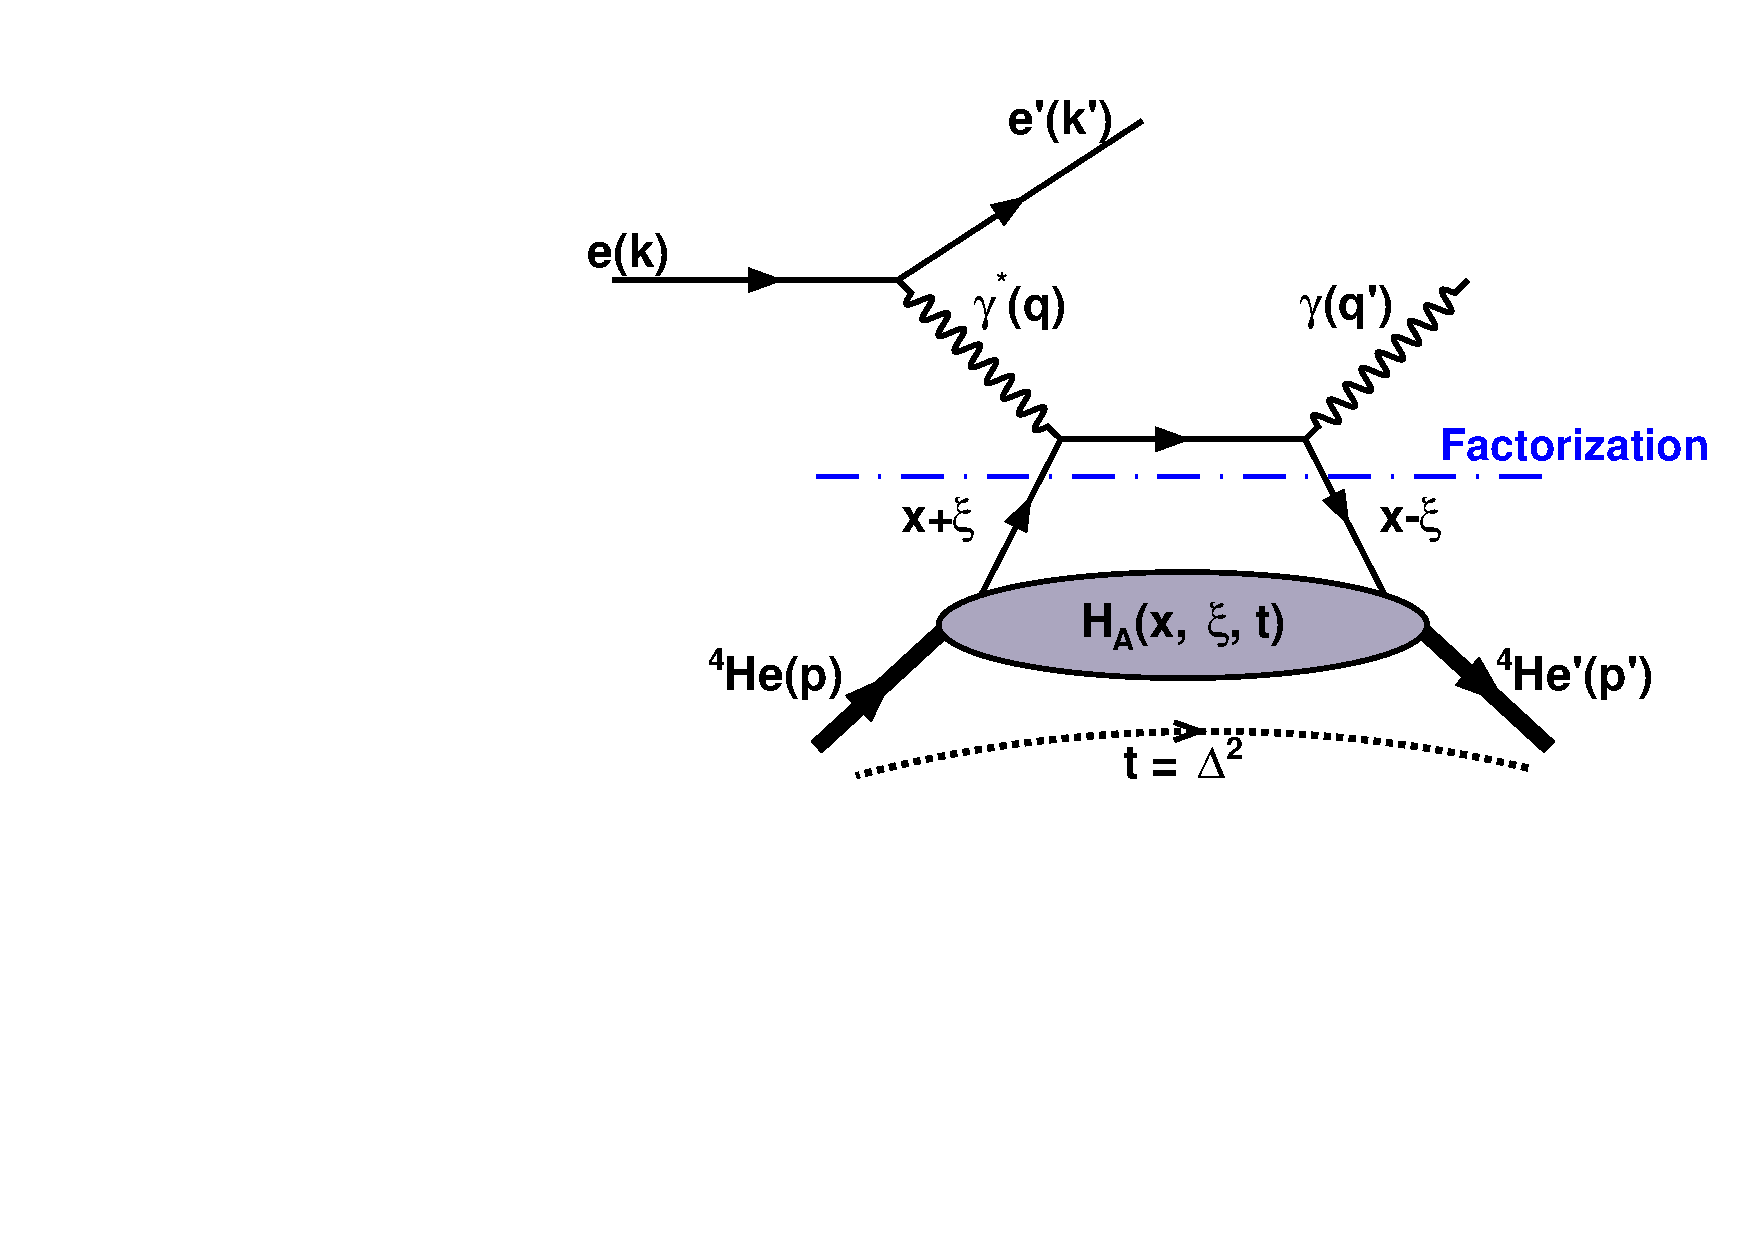
\includegraphics[width=9cm]{fig3/DVCS_diagram.pdf}
\caption{Diagram representing the coherent nuclear DVCS.}
\label{fig:CohDiag}
\end{figure}
%TODO fix delta

This formula can be expressed in a simplified manner for a spin-0 target as \cite{Belitsky:2008bz}:
\begin{equation}
A_{LU}(\phi) = \frac{\alpha_{0}(\phi) \, \Im m(\mathcal{H}_{A})}
{\alpha_{1}(\phi) + \alpha_{2}(\phi) \, \Re e(\mathcal{H}_{A}) + \alpha_{3}(\phi) \, 
\big( 
\Re e(\mathcal{H}_{A})^{2} + \Im m(\mathcal{H}_{A})^{2} \big)}
\label{eq:A_LU-coh}
\end{equation}
where $\Im m(\mathcal{H}_{A})$ and $\Re e(\mathcal{H}_{A})$ are the imaginary 
and real parts of the CFF $\mathcal{H}_{A}$ associated to the GPD $H_A$ of the 
spin-0 nucleus. The 
$\alpha_{i}$ factors are $\phi$-dependent kinematical terms that depend on the 
nuclear form factor $F_A$ and the independent variables $Q^2$, $x$ and $t$.  
These factors have the following simplified expressions:
%\small
\begin{eqnarray}
	\label{eq:alpha1}
   \alpha_0 (\phi) & = &\frac{x_{A}(1+\epsilon^2)^2}{y} S_{++}(1) \sin(\phi)\\
    \alpha_1 (\phi) & = & c_0^{BH}+c_1^{BH} \cos({\phi})+c_2^{BH} \cos(2\phi)\\ 
   \alpha_2 (\phi) & = & \frac{x_{A}(1+\epsilon^2)^2}{y}  \left( C_{++}(0) +  
C_{++}(1) cos(\phi) \right)\\
\alpha_3 (\phi) &=& \frac{x^{2}_{A}t(1+\epsilon^2)^2}{y} {\mathcal P}_1(\phi) 
{\mathcal P}_2(\phi) \cdot 2 \frac{2-2y+y^2 + \frac{\epsilon^2}{2}y^2}{1 + 
\epsilon^2},
	\label{eq:alpha4}
\end{eqnarray}
%\normalsize
where $S_{++}(1)$, $C_{++}(0)$, and $C_{++}(1)$ are the Fourier harmonics in the 
leptonic tensor \cite{Belitsky:2008bz} and $x_{A} = \frac{M_{p}\cdot x}{M_{^4\!He}}$. 
%Their explicit expressions can be found in Appendix 
%\ref{app:Helium_cross_section}.  

The Eq. \ref{eq:A_LU-coh} is particularly convenient to perform an extraction of 
the $\Im m(\mathcal{H}_{A})$ and $\Re e(\mathcal{H}_{A})$ through a fit of the BSA as 
a function of $\phi$. As can be seen in Fig. \ref{fig:alphas}, the form of each 
$\alpha$ coefficient is known and characteristic, such that a fit is easy. The only caveat
is the large difference of magnitude between the $\alpha$ factors, which will lead to 
rather different error propagation for the two parts of the CFF.

\begin{figure}[tbp!]
\center
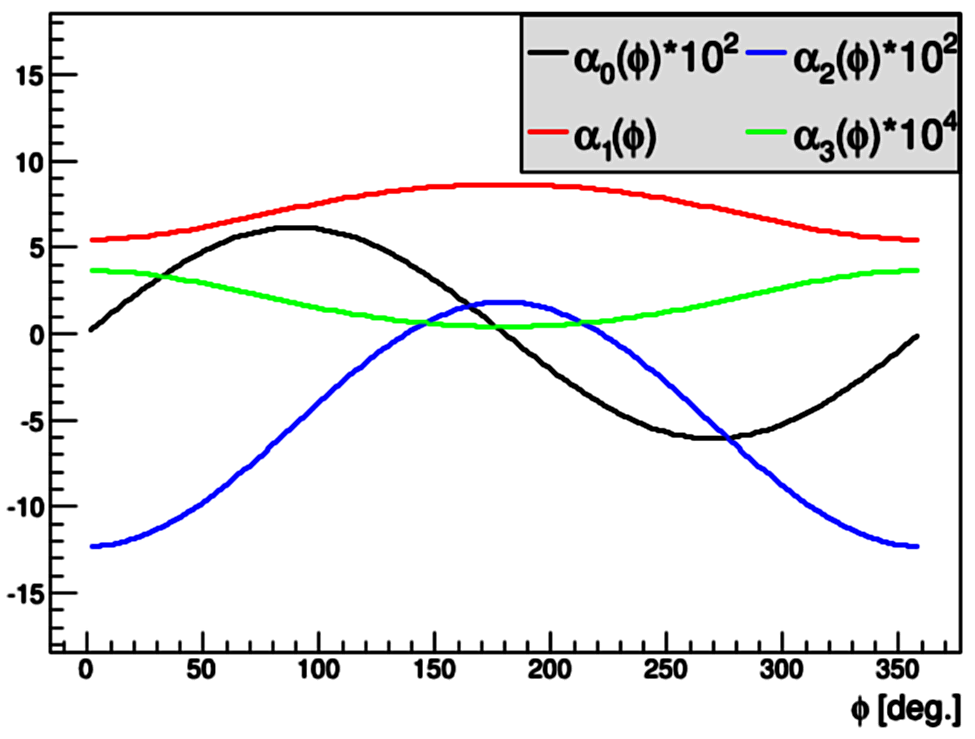
\includegraphics[width=8cm]{fig3/AlphaCoefs.png}
	\caption{Coefficients presented in Eq. \ref{eq:alpha1} to \ref{eq:alpha4}.
	Note the prescaling factors used for $\alpha_0$, $\alpha_2$ and $\alpha_3$.}
\label{fig:alphas}
\end{figure}

\subsection{Incoherent nuclear DVCS}

The incoherent nuclear DVCS process, is the DVCS off a bound nucleon in a nucleus
as represented in Fig. \ref{fig:InCohDiag} for an helium-4 target. The remnants of 
the nucleus ($X$) contain only the missing three nucleons. 
The theory for incoherent DVCS on the nucleon is largely based on the free proton theory
already reviewed in Chap. \ref{chap:pheno}. Two important differences in the 
reaction need to be accounted however, the different initial state and the addition of 
final state effects. In the initial state, the intrinsic Fermi motion of the nucleons in the nucleus 
lead to an uncertainty on the exact kinematic of the reaction. Moreover, in general the nucleon 
is in an off-shell state that is not exactly identical to its final state. In the final state, 
interactions between the outgoing nucleon from the DVCS reaction and remnants of the nuclear 
target are possible, including possible charge exchange. The latter
leading to contamination from other channels, in particular charge exchange can lead to
large differences in this background. 

\begin{figure}[tbp!]
\center
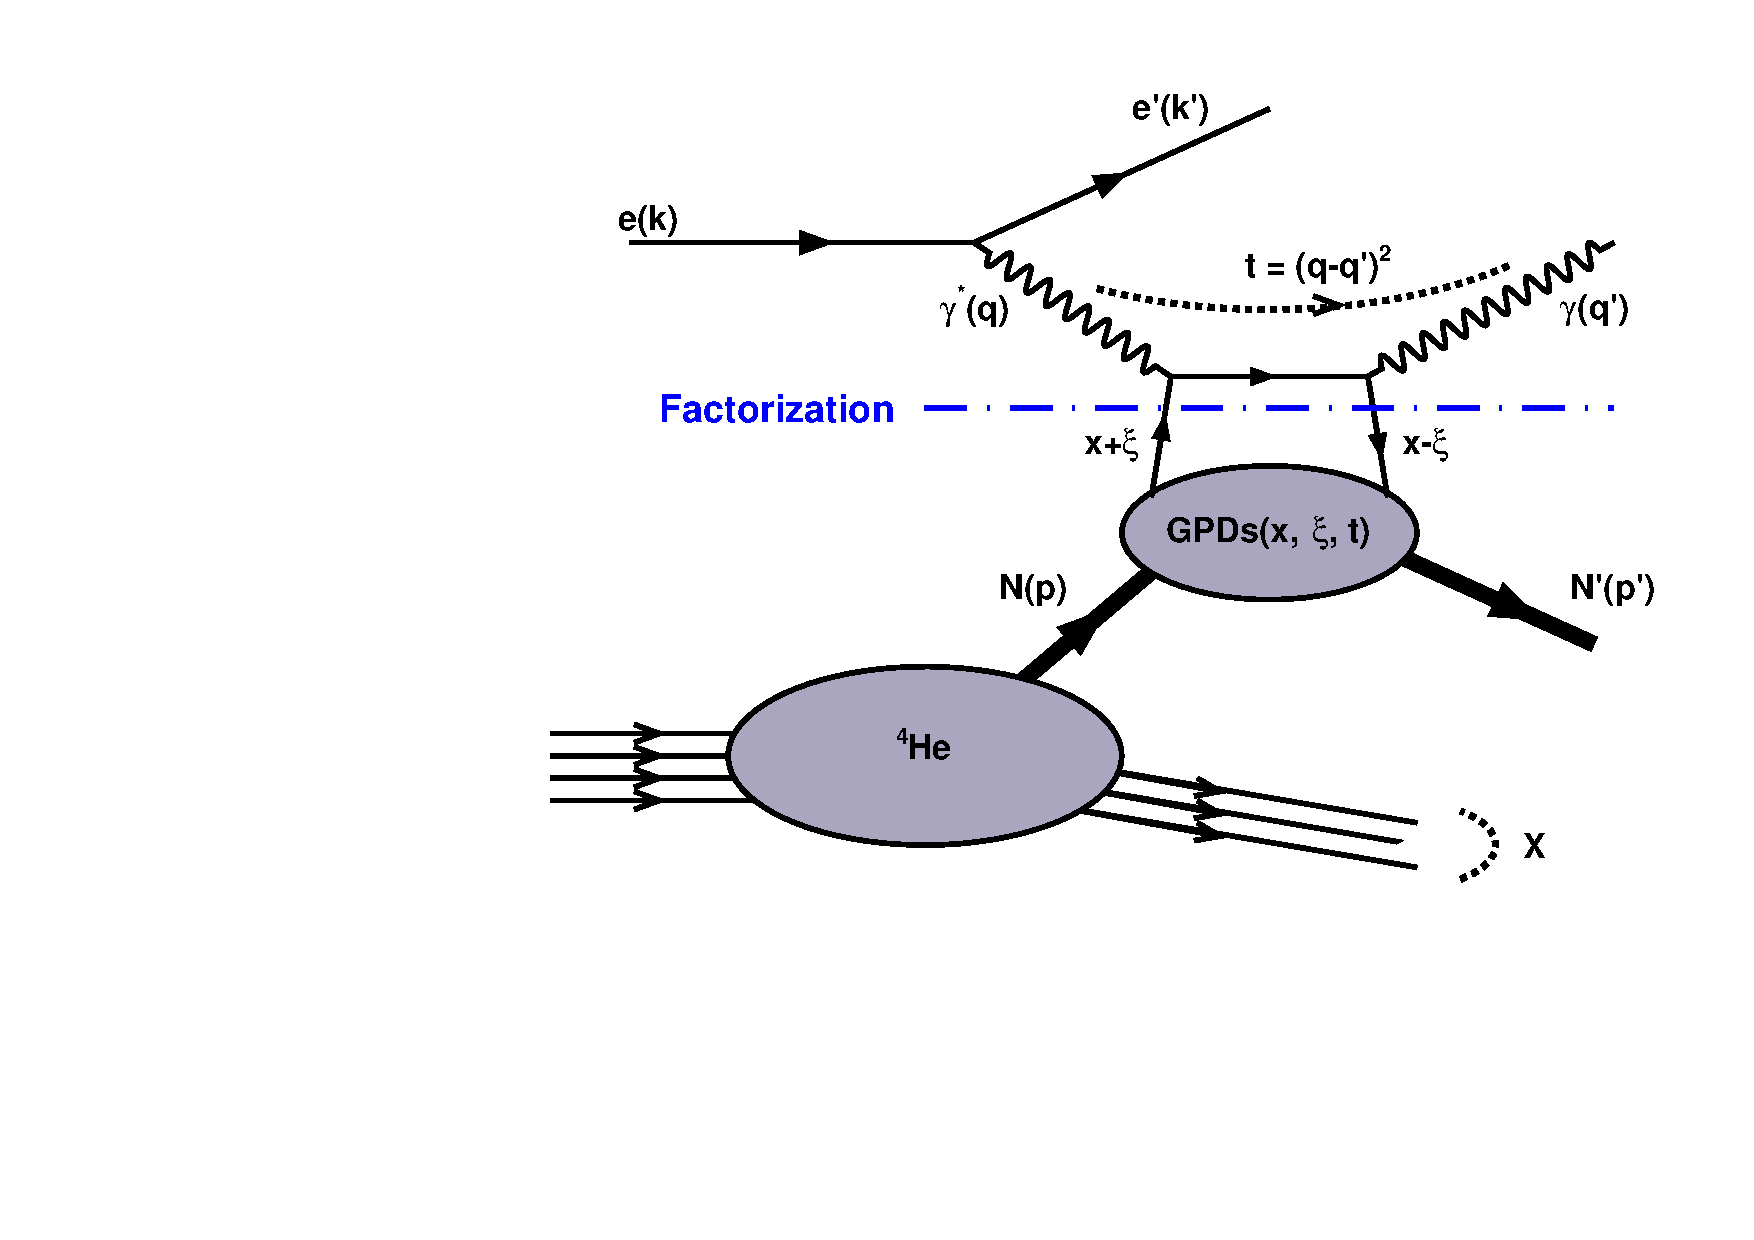
\includegraphics[width=10cm]{fig3/handbag_incoherent.pdf}
\caption{Diagram representing the incoherent nuclear DVCS.}
\label{fig:InCohDiag}
\end{figure}

Since, DVCS is a 
process selected using tight exclusivity constrains, some of the initial and final-state effects are
automatically mitigated. Selection criterion on missing energy and momentum are performed,
constraining the range of initial Fermi motion and final interactions possible. However, no theoretical
calculation is available to correct for the reminder of these effects yet. Since, modern calculations exist 
for such effects in DIS \cite{Cosyn:2017ekf}, we can expect them to be extended to the DVCS 
process as more data becomes available. Another avenue of progress
on this topic will be the use of experimental techniques like tagging to control them. This process
and how it can help with these issues will be discussed
in details at the end of the present chapter.

\subsection{The HERMES nuclear DVCS measurements}

The first measurement of nuclear DVCS has been performed by the HERMES collaboration 
\cite{Airapetian:2009cga}.
This experiment covered an array of nuclear target and looked at the $A$ dependence of the
BSA signal. The results, presented in Fig. \ref{fig:HERMES1} and \ref{fig:HERMES2}, suffer
from large error bars, which makes them consistent with the free proton data and prevents us to
reach strong conclusions about the nuclear effect. Yet, in the coherent DVCS case a rather
strong effect was expected, leading to a conflict between the HERMES results and theoretical
expectations. 

\begin{figure}[tbp!]
\center
	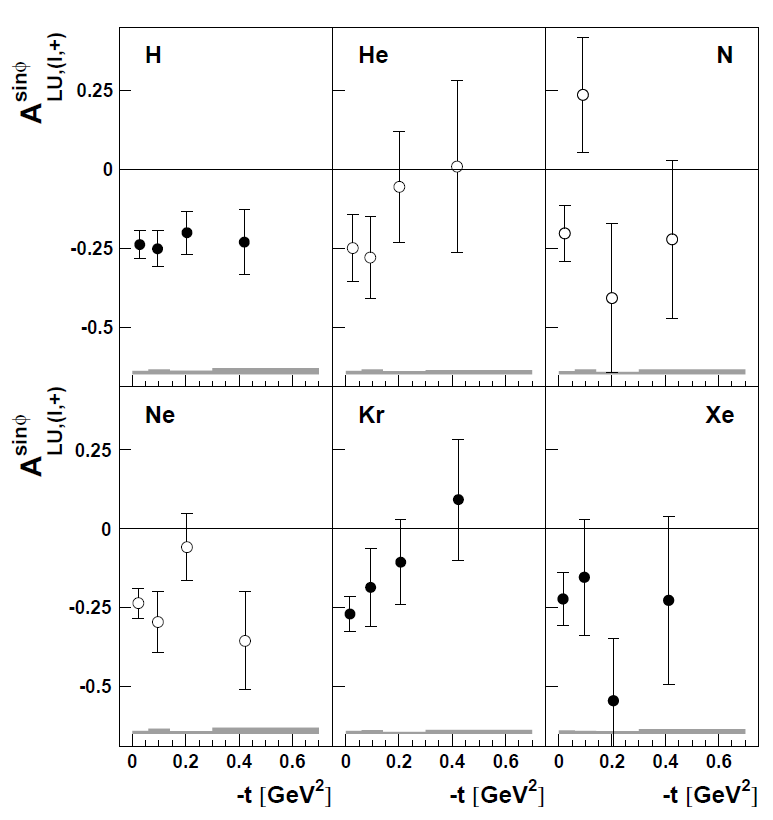
\includegraphics[width=10.5cm]{fig3/HERMES_BSA.png}
	\caption{The sinus moment of the BSA as a function of $-t$ measured by HERMES
	on a series of nuclei \cite{Airapetian:2009cga}.}
\label{fig:HERMES1}
\end{figure}

\begin{figure}[tbp!]
\center
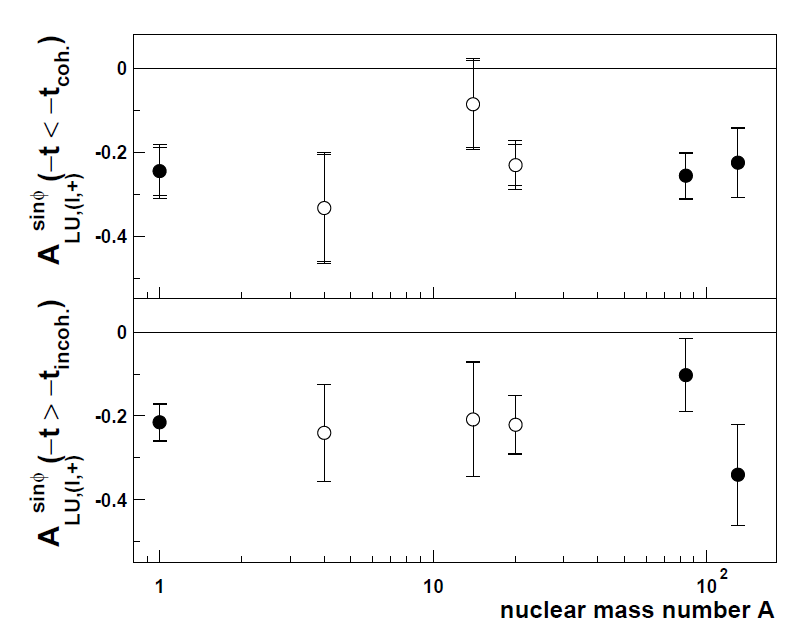
\includegraphics[width=10cm]{fig3/HERMES_BSA_2.png}
\caption{The sinus moment of the BSA at low and high $-t$ as a function of $A$ measured by HERMES
	\cite{Airapetian:2009cga}.}
\label{fig:HERMES2}
\end{figure}

An issue with the HERMES measurement and how it is obtained from data has been raised in
\cite{Guzey:2003jh} to explain the discrepancy with theoretical expectations.
The main concern is that the DVCS process is not fully detected and the scattered target
is instead reconstructed through a missing mass measurement of the other reaction products. The 
issue with this method is that the detector resolution is not good enough to separate the 
coherent and incoherent channels. 
Instead, the results are labeled "coherent enriched" and "incoherent enriched" at low and high 
$-t$, respectively. This label is based on the assumption that the very different behavior of the
cross sections of the two channels in $t$ will lead to a clear differentiation. However, the
results in Fig. \ref{fig:HERMES2} show similar behaviors in both sectors of $t$, which is 
challenging this assumption and could explain the tension between theory and experiment. 

Altogether, the large error bars and the impossibility to properly separate the coherent and 
incoherent channels have strongly impaired the measurement and any conclusions that could be
obtained from it. The CLAS experiment presented here has profited largely from this
result and was designed specifically to solve these two issues of low statistics and exclusivity.

\section{The CLAS nuclear DVCS experimental setup}

The CLAS experiment had for main objective to explore the coherent DVCS on helium-4 and assess if
the predicted BSA increase could be observed and if GPDs could be extracted from it. In order to
perform this measurement however, several instrumentation challenges need to be passed. First, to
measure the scattered electron and the low angle photon of the DVCS, for which we used CLAS in its 
DVCS setup, $i.e.$ with the addition of a low angle calorimeter and a solenoid magnet. Second, the
helium recoil need to be measured to ensure the exclusivity of the reaction. In this section, we 
will rapidly describe the particular detector setup used in our experiment. 

\subsection{The CLAS detector}

CLAS is installed in the hall B of the JLab main accelerator. It has for main objective to study the 
multi-particles final states
that cannot be reconstructed with arm spectrometers. Its historic use to measure DVCS in many different 
configurations made it an ideal place for this new DVCS measurement.  

The CLAS spectrometer \cite{Mecking:2003zu} is composed of six identical radial 
sectors separated by a toroidal magnet and each sector is made of four detectors 
as shown in Fig. \ref{fig:CLAS}.  Three regions of drift chambers \cite{Mestayer:2000we} 
are placed in the solenoid area to reconstruct the charge particle's tracks and 
calculate their momentum. Then, an array of scintillators is placed to measure 
a precise time for each track and perform time-of-flight measurement 
\cite{Smith:1999ii}. These detectors cover the polar angle from 8 to 142 degrees. 
This is completed by two important forward detectors, from 8 
to 45 degrees for electron identification, a Cerenkov counter 
\cite{Adams:2001kk} and an electromagnetic calorimeter \cite{Amarian:2001zs}. 

\begin{figure}[tbp!]
\center
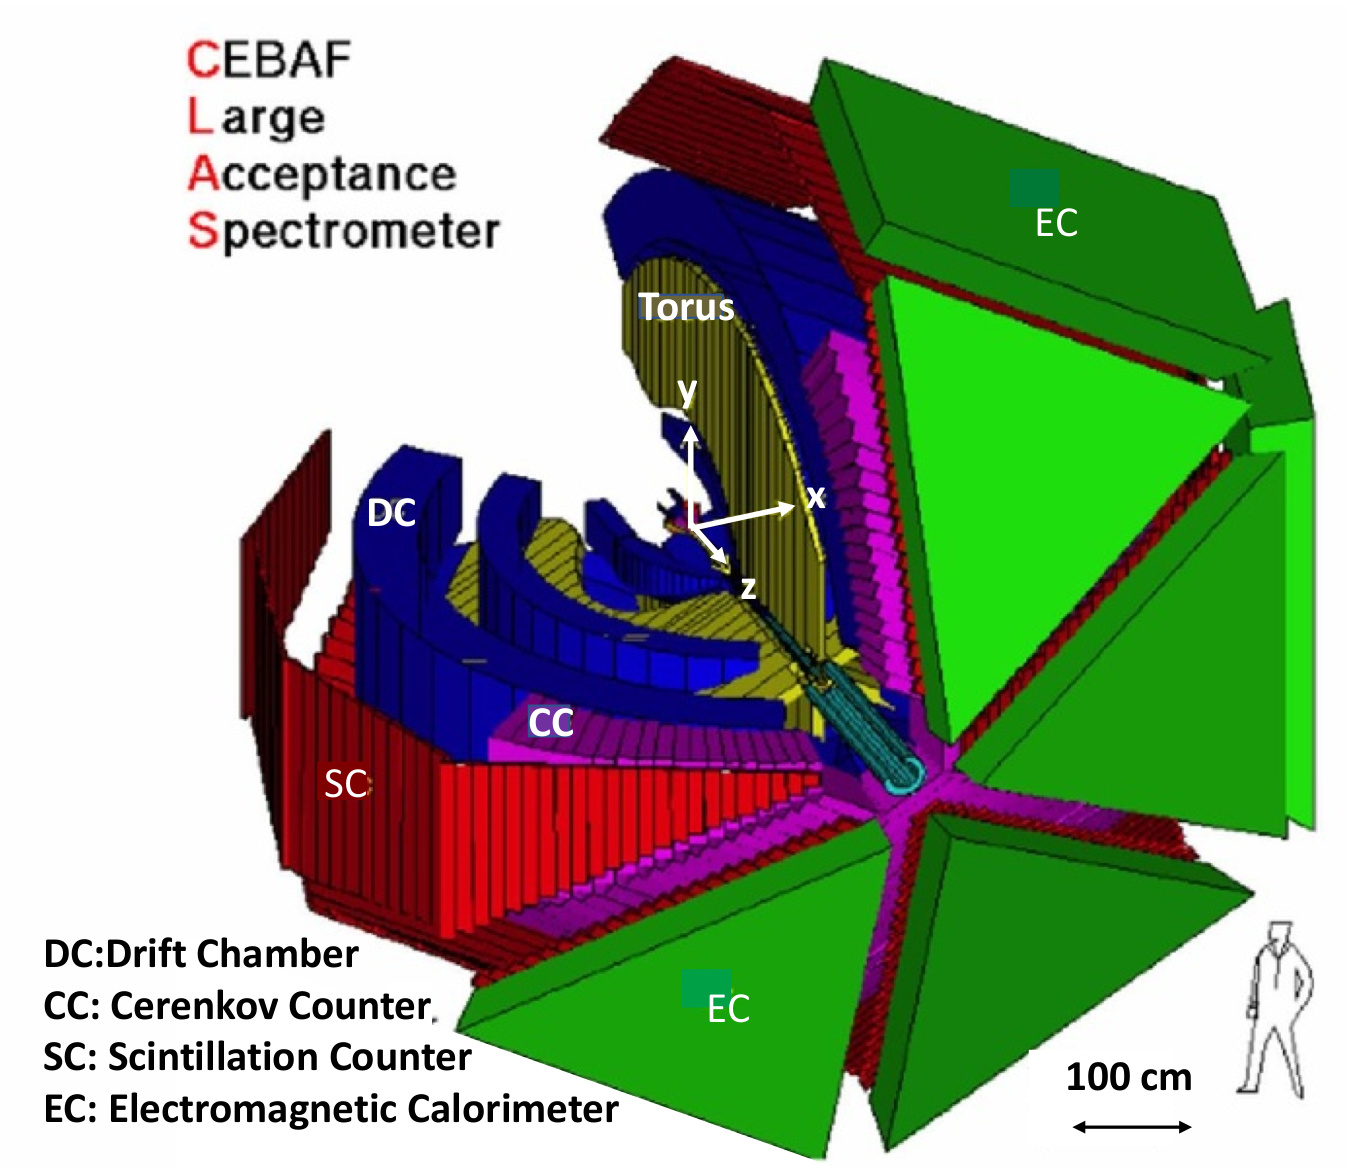
\includegraphics[width=8cm]{fig3/CLAS_geantview-PS.jpg}
	\caption{View of the CLAS detector setup.}
\label{fig:CLAS}
\end{figure}


Altogether, CLAS provides a large acceptance of about $\pi$ steradians for momentums 
starting at 200 MeV/c. During the nuclear DVCS experiment,
the beam energy was maximal for CLAS with 6.064 GeV, while the beam intensity varied
between 120 and 150 nA. Such beam on our helium-4 target pressurized between 5 and 6 atm,
corresponds to luminosities in the range of $1$ to $1.2 \times 10^{34}$ cm$^{-2}$.s$^{-1}$.
During the experiment, the data acquisition rate ran around 3 kHz with about 70\% live-time
using an inclusive electron trigger. 

\subsection{Adaptations for DVCS}

The CLAS collaboration has established a specific setup to measure the typically 
low angle photons of the DVCS process. This setup is composed of an inner 
calorimeter and a solenoid and has lead to numerous DVCS measurements on proton 
targets \cite{Seder:2014cdc,Jo:2015ema,HirlingerSaylor:2018bnu}.

The inner calorimeter, illustrated in Fig. \ref{fig:IC} is a homogeneous 
calorimeter composed 424 lead tungstate 
(PbWO) crystals read out by $5 \times 5$ mm$^2$ avalanche photo-diodes (APDs). 
It covers angles from 4 to 15 degrees. However, placing a detector at such low angles makes it 
particularly sensitive to the Moller electrons scattered at low angles.

\begin{figure}[tbp!]
\center
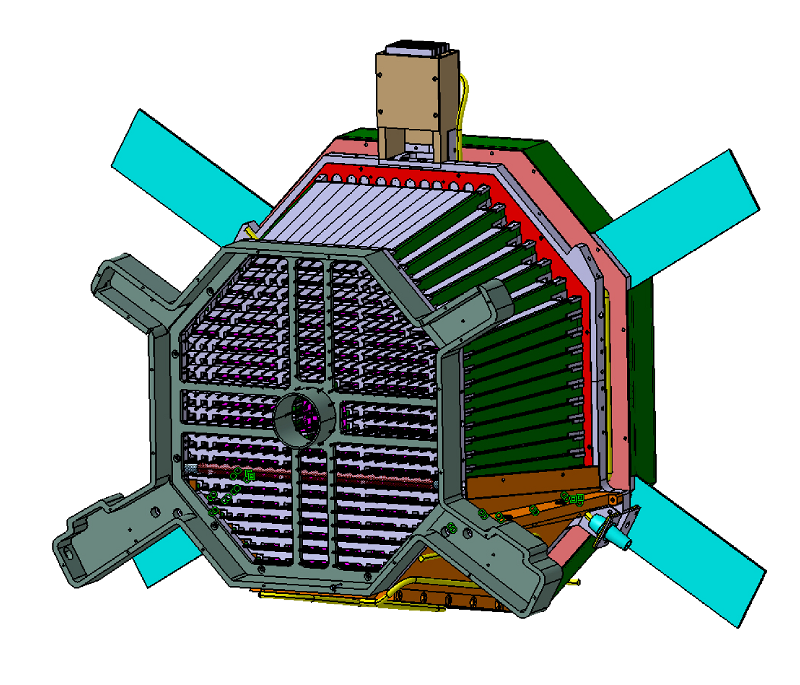
\includegraphics[width=8cm]{fig3/IC-CLAS.png}
	\caption{Representation of the inner calorimeter (IC) of CLAS. The crystals that compose the
	sensitive part of the detector are represented in purple.}
\label{fig:IC}
\end{figure}

To protect the calorimeter from the low energy background a 5~T solenoid is 
placed around the target to form
a magnetic shield. Thanks to this field, low energy charged particles (particularly 
electrons) curl around the beam line 
and never make it to the calorimeter or other CLAS detectors as illustrated 
by simulation results presented 
in Fig. \ref{fig:Solenoid}. This allows to run much higher luminosity experiments,
a necessity for low rates processes like DVCS.

\begin{figure}[tbp!]
\center
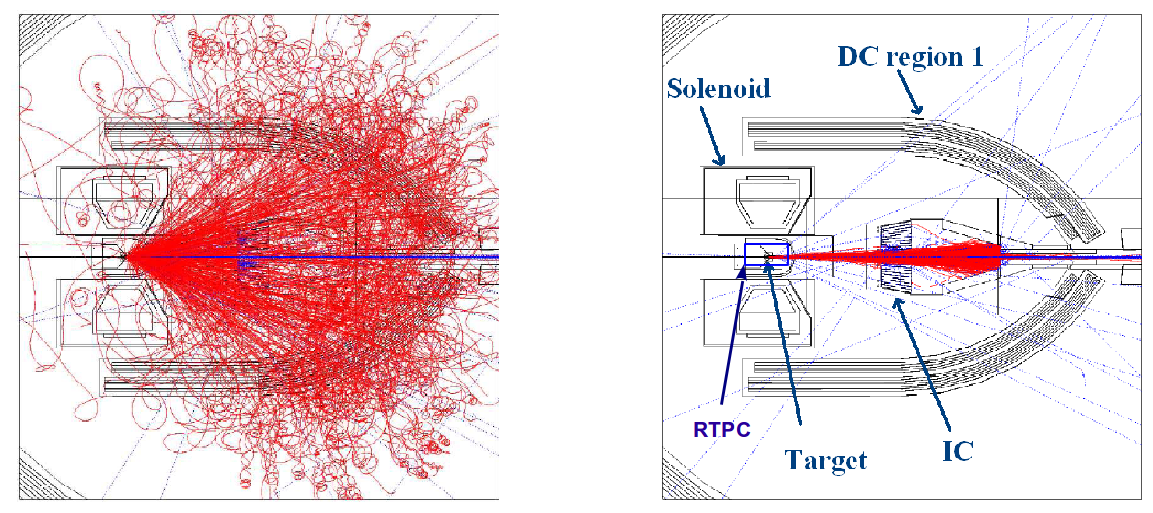
\includegraphics[width=14cm]{fig3/solenoid.png}
\caption{Representation of the center of CLAS with the beam background in red with and without
	the solenoid field activated, right and left, respectively.}
\label{fig:Solenoid}
\end{figure}


\subsection{The Radial time projection chamber}

The recoil helium nuclei from coherent DVCS are mostly emitted between 150 
and 200 MeV/c at our beam energy. Therefore, a specific detector was 
needed to detect them. To design the present setup, large inspiration was drawn from the 
Bonus setup that also used a GEM based RTPC \cite{Fenker:2008zz}, installed in CLAS to 
detect slow protons out of a deuterium target \cite{Baillie:2011za}. In such an RTPC the 
charges are projected toward large radii 
rather than towards the endcaps, as is more traditional in time 
projection chambers. This design allows to reduce significantly the drift time and reduce the 
amount of pile-up from accidental events. The RTPC has been described in more 
details elsewhere \cite{Dupre:2017upj}, here is a summary of key elements.

In order to detect the recoil helium nuclei from a DVCS reaction, we first need 
to ensure that it will come out of the target. For this, we used a light straw 
target made of a thin kapton wall of 27 $\mu$m filled with up to 6 atm of 
helium. The entrance and exit windows are thin aluminum foils and an helium 
bag is placed downstream of the target to avoid interaction with air in the gap 
between the target and the beamline vacuum. The cylindrical 
chamber surrounds the target as illustrated in Fig. \ref{fig:RTPCGlobal}, we 
list the elements composing it based on their radii:
\begin{itemize}
	\item Up to a radius of 3 mm the pressurized helium target.
	\item From 3 to 20 mm a keep-out zone filled with 1 atm of helium to 
		minimize the production of secondaries. 
	\item At 20 mm a grounded foil made of 4 $\mu$m aluminized Mylar to 
		isolate the chamber from the beam line 
		region and collect charges. It also serves to separate gas regions.
	\item From 20 to 30 mm a dead zone to separate the ground from the cathode
		filled with the drift gas, a mix of neon and dimethyl ether (DME) in 
		80/20 proportions.
	\item At 30 mm the cathode foil made of 4 $\mu$m aluminized Mylar.
	\item From 30 to 60 mm the drift region filled with the drift gas.
	\item From 60 to 69 mm the amplification regions, filled with drift gas, 
		with GEM foils placed at 60, 63 and 66 mm.
	\item At 69 mm the collection pads connected to the preamplifers placed 
		directly outside the chamber.
\end{itemize}

\begin{figure}[tbp!]
\center
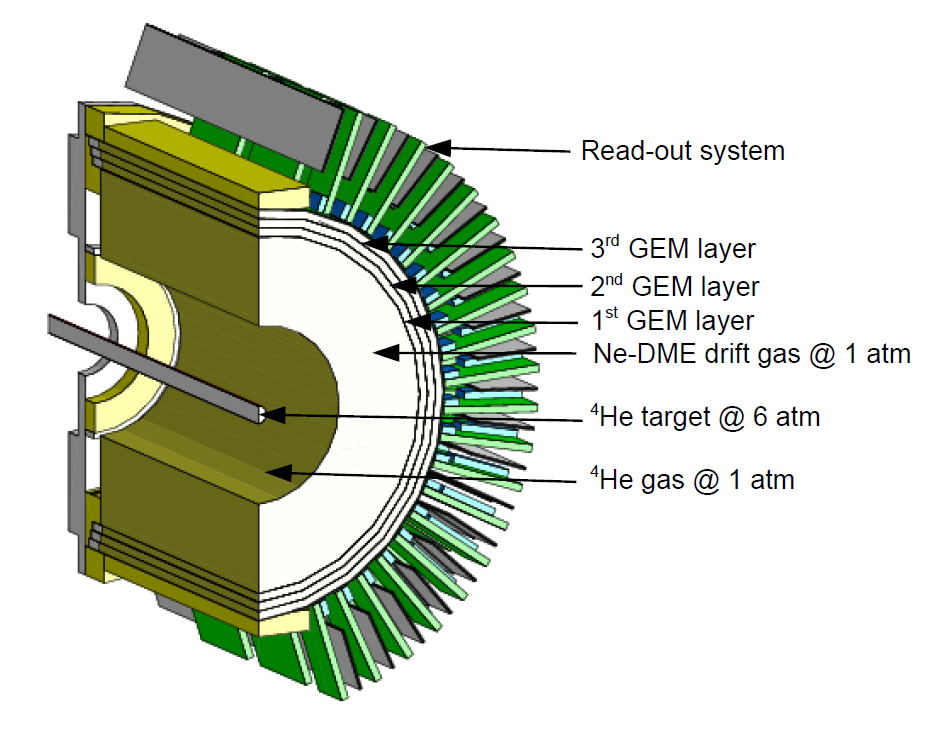
\includegraphics[width=10cm]{fig3/RTPC_new_1.png}
\caption{Cut view of the RTPC.}
\label{fig:RTPCGlobal}
\end{figure}

The calibration of the detector has been performed with a 
dependence on $z$, the position along the beam line axis, due to 
variations in the magnetic fields. To perform this calibration we took  
dedicated data at 1.2 GeV beam energy. In 
this data set, we were able to select elastic events, for which the kinematic 
of the helium recoil can be calculated from the electron kinematic and 
directly compared to the measurement in the RTPC. This comparison helped to 
map the correspondence between time and position in the chamber and determine 
the drift path of electrons. A more detailed description of the calibration process 
is available in \cite{Dupre:2017upj}.

\section{DVCS event selection}

\subsection{Particle identification}

The electrons are detected with the baseline CLAS detectors, the drift chamber measures the kinematic 
of the electron and the large signal in both the Cerenkov counter and electromagnetic calorimeter
provide the identification. A signal of good quality is also required in the 
time-of-flight system, which serves as a time reference for other detectors. In particular, it 
serves for the identification of the protons, which is based on a 
time-of-flight measurement. Several 
fiducial cuts are applied to ensure that particles did not go through part of the inner calorimeter 
or the solenoid, as well as to reject the edges of the detectors, where efficiency is rapidly 
decreasing. Kinematic corrections are also applied to the electrons and protons to correct for energy loss
and biases in calibration, they are at subpercent level except for protons below 500 MeV/c for which they
go up to 10\% at the detection limit of 200 MeV/c.

The photons from DVCS are mainly detected with the inner calorimeter. No specific 
identification cuts are used in this detector as large energy deposit are dominantly 
from electrons and photons, which cannot be separated reliably. However, the detection 
of an electron at larger angle in CLAS 
highly suppresses the number of electrons in the calorimeter, moreover
the exclusivity cuts used later in the analysis further this suppression. Left over accidentals, will be
accounted for in the background subtraction. The inner calorimeter was calibrated through a series
of steps, involving the reconstruction of $\pi^0$ from their two photons decay. Calibration was obtained 
with an iterative process to adjust each crystal gain to obtain the most accurate $\pi^0$ mass. A
global calibration of the calorimeter was also performed to account for incident angle, energy and 
time dependent effects.

Finally, we select events that contain a single electron, a high energy photon ($E>2$ GeV) and
either a helium or a proton. We perform a vertex selection cut on the two charged particles 
to ensure they originate from the same vertex, inside the target, thus rejecting target windows.
Moreover, since we are aiming to study deep processes occurring at the partonic level, we select
$Q^2>1$ GeV$^2$. Also, the transferred momentum squared to the recoil $^{4}He$ is bound by
   a minimum value based on basic energy momentum conservation:
\begin{equation}
   t_{min} = - Q^{2} \frac{2(1- x_{A})(1 - \sqrt{1 + \epsilon ^{2}}) + \epsilon 
   ^{2}}{4 x_{A}(1-x_{A})+ \epsilon ^{2}},\\
\end{equation}
where $\epsilon ^{2} = \frac{4M^{2}_{^4\!He}x^{2}_{A}}{Q^{2}}$. For incoherent DVCS, 
$x_A$ is replaced by $x$ and $M_{^4\!He}$ by $M_{p}$. 

\subsection{Exclusive photo-production selection}

To select exclusive events and suppress the backgrounds, we define several 
exclusivity cuts based on energy and momentum conservation. In principle, 
a selection based on two or three variables can be used to guaranty the 
exclusivity of the process. However, in such experiment, where particles 
are detected at very different energies and with very different detector 
precision, we chose to over constrain the selection by using seven 
variables. The seven variables are defined as follow for the coherent 
DVCS (replace helium by proton for the incoherent case):
\begin{itemize}
	\item Co-planarity ($\Delta \phi$) of the virtual photon, the real photon and
		the recoil helium, defined as the angle between the helium, virtual photon
		plane and the virtual photon, real photon plane;
	\item Missing energy of the full system;
	\item Missing mass of the full system;
	\item Missing transverse momentum of the full system;
	\item Missing mass of the system electron-helium, ignoring the photon;
	\item Missing mass of the system electron-photon, ignoring the recoil helium;
	\item Co-linearity ($\theta$) of the measured photon with the missing momentum of the 
		electron-helium system.
\end{itemize}

In the analysis, we apply selection cuts based on a fit of the exclusive peak at 3$\sigma$ around 
the mean value for each variable. This automatic method helps to avoid any bias 
in the selection of the events. The selection of coherent DVCS with these variables is illustrated in 
Fig. \ref{fig:CohExcCuts}. We note on these distributions only few minor anomalies, where the 
distribution have some asymmetries. These are linked with the detector resolutions, that impact
differently the kinematic variables. The selection of incoherent DVCS is presented in 
Fig. \ref{fig:IncExcCuts}, with two main differences: larger distributions overall and more
offset distributions. The former is largely due to Fermi motion, but simulations have shown
that this effect is not strong enough to reproduce these distribution widths and final 
state interactions must play a role as well. The later is caused by slight detector 
misalignment between CLAS sectors and are within the levels obtained with free proton 
targets to which they can be directly compared (see \cite{HirlingerSaylor:2018bnu} for instance). 

\begin{figure}[tbp!]
\center
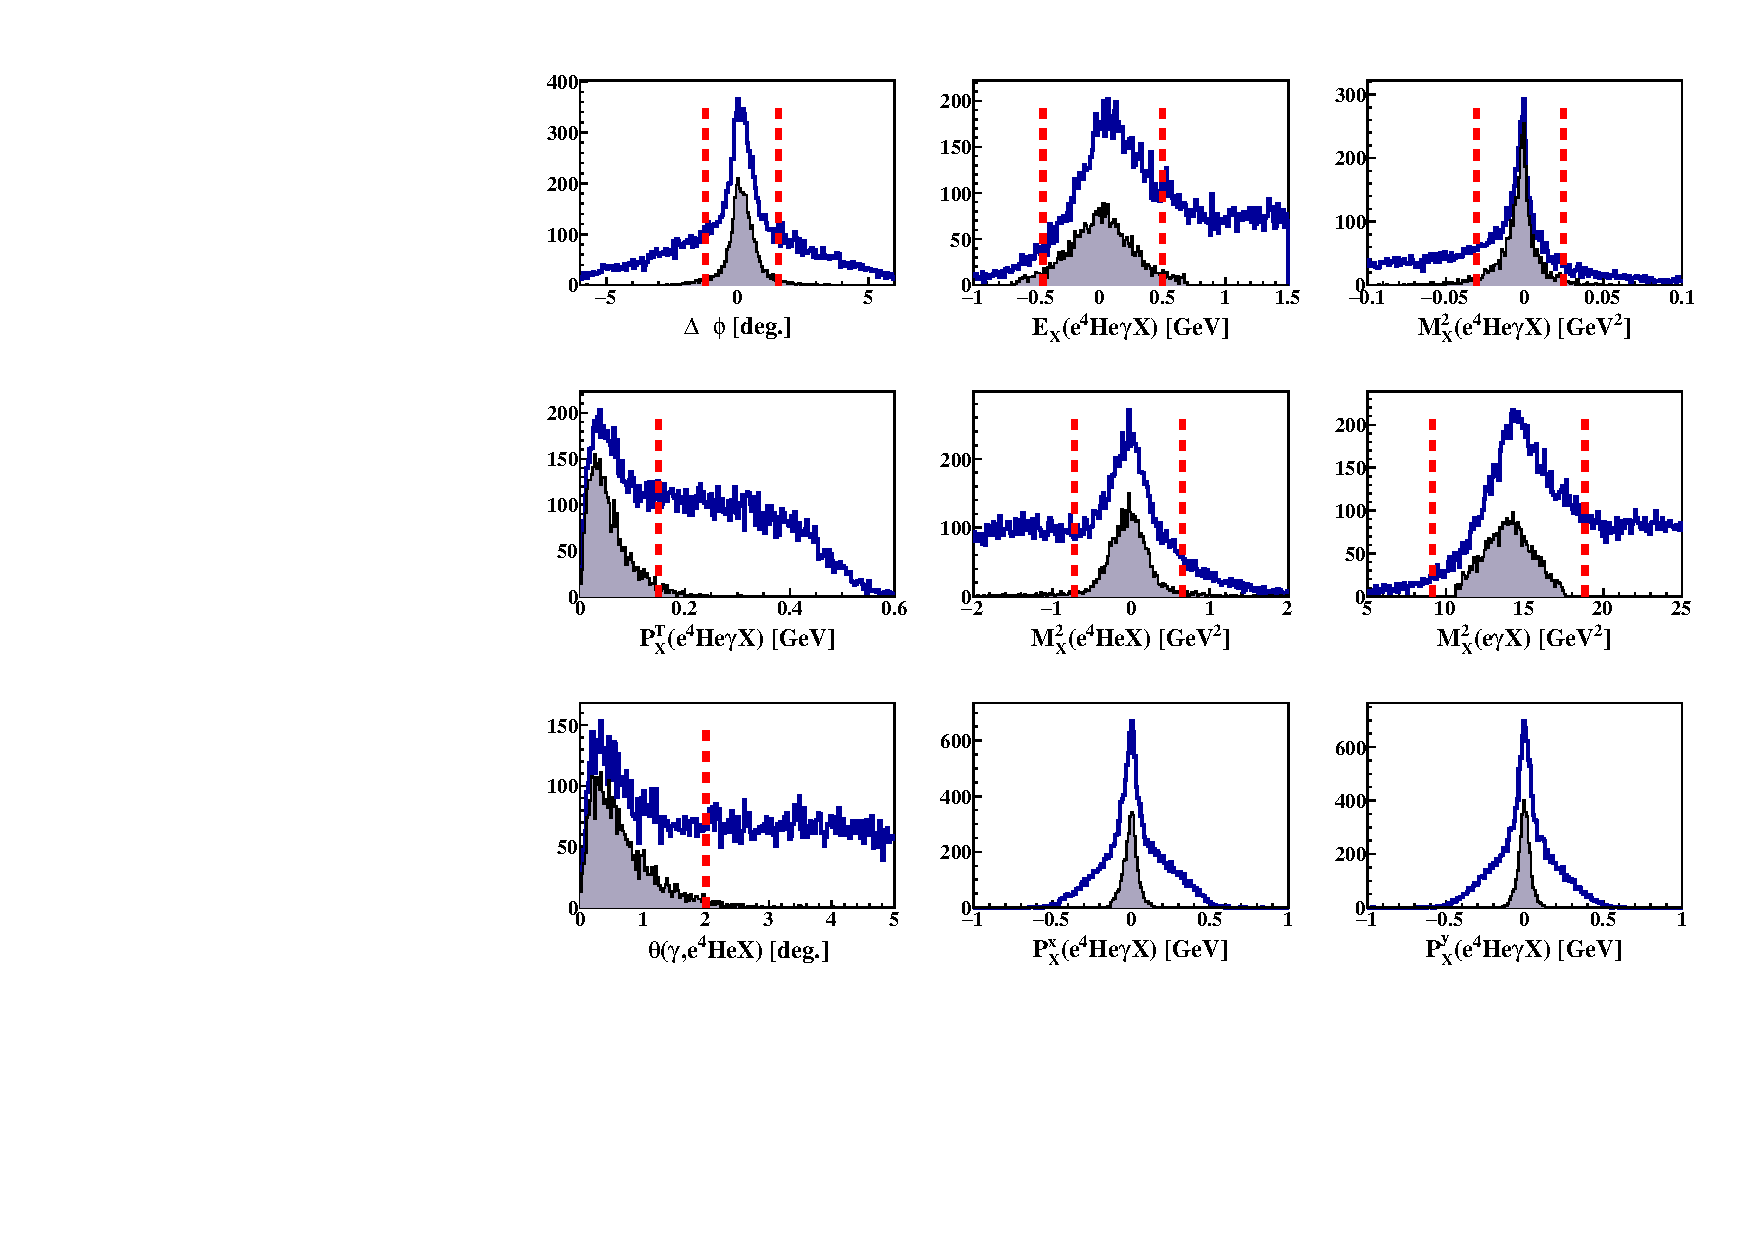
\includegraphics[trim=20 10 20 5,clip,width=15cm]{fig3/all_coh_exc_cuts.pdf}
	\caption{Overlay of the events distributions before (black) and after (blue line filled
	in Grey) the exclusivity cuts used to select coherent DVCS represented by the 
	red dashed lines. The histograms are for the seven variables described in the text, 
	plus the missing $P_x$ and $P_y$, in order left to right and top to bottom.}
\label{fig:CohExcCuts}
\end{figure}

\begin{figure}[tbp!]
\center
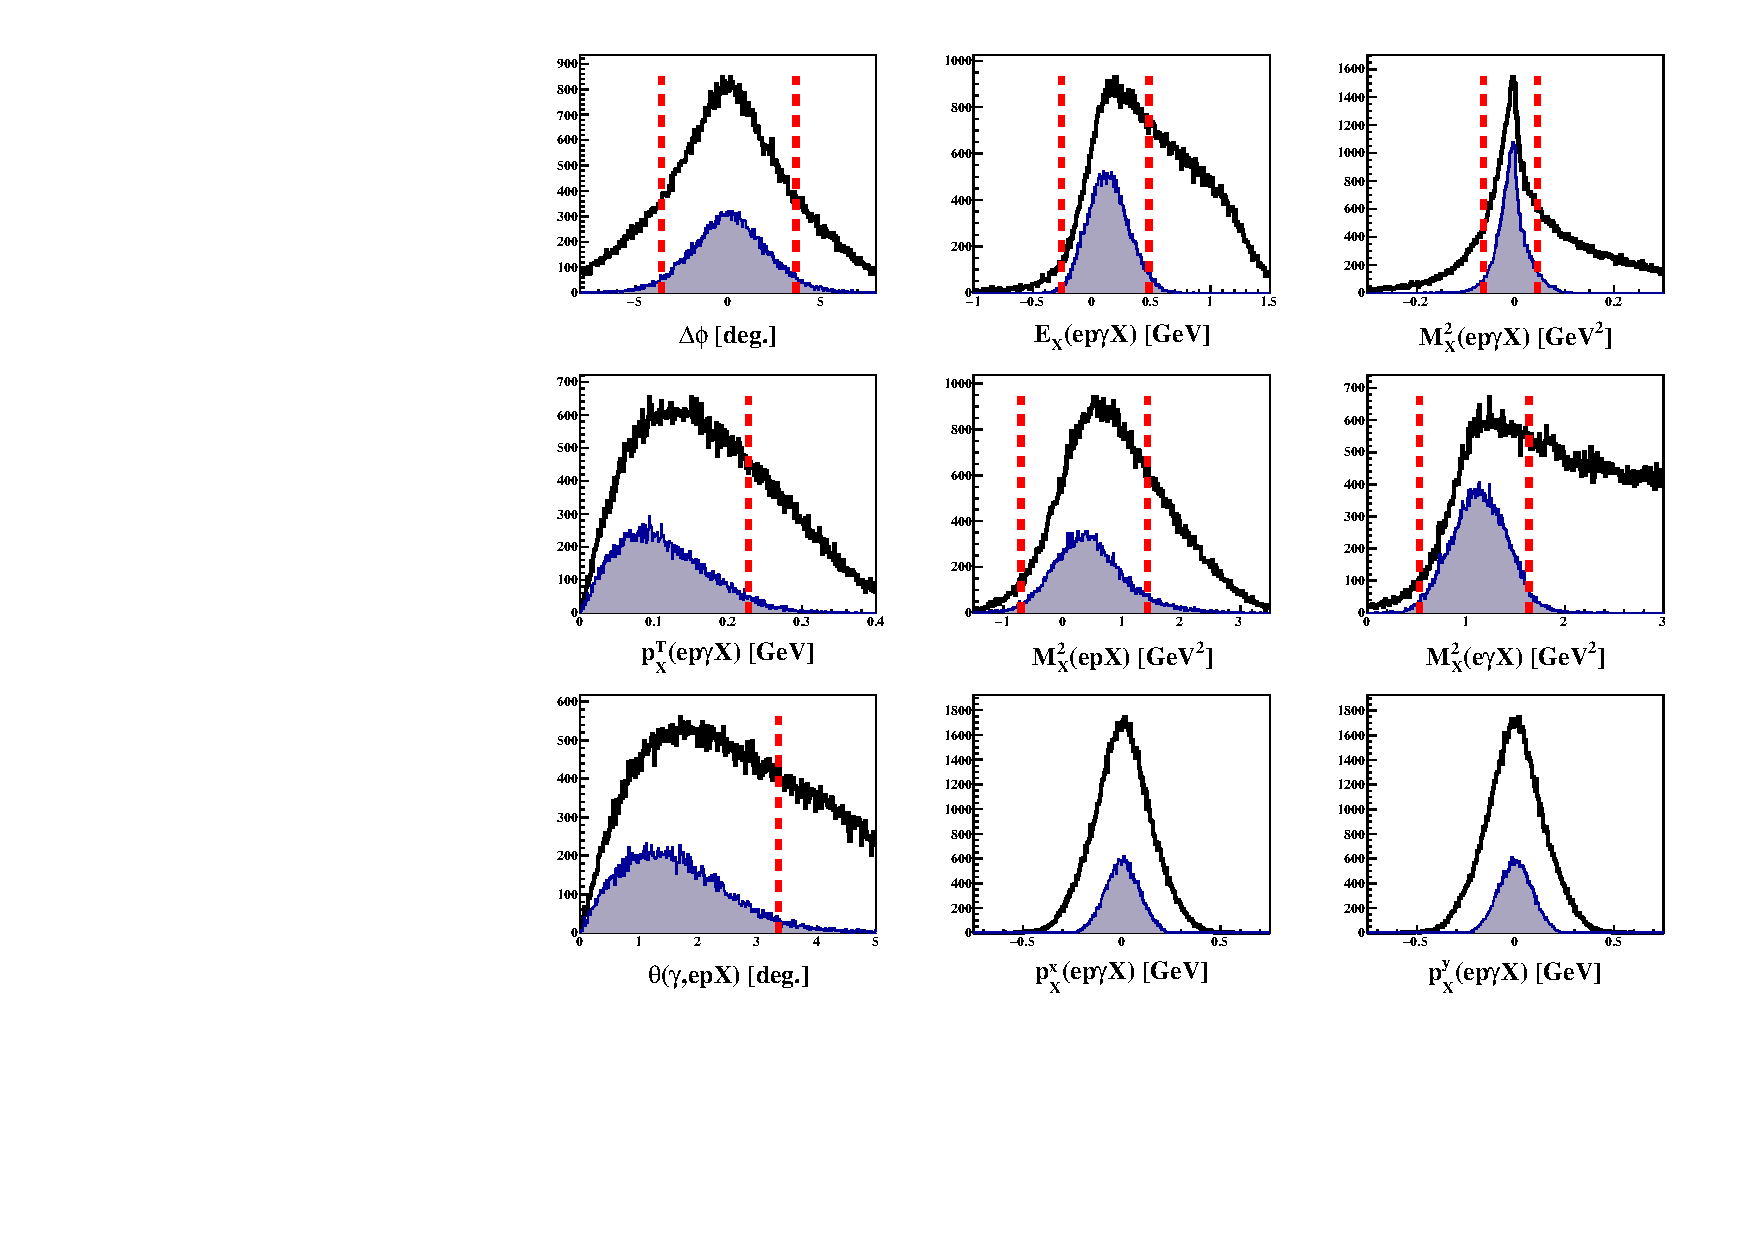
\includegraphics[trim=20 10 20 5,clip,width=15cm]{fig3/all_incoh_exc_cuts.pdf}
\caption{Overlay of the events distributions before (black) and after (blue line filled
	in Grey) the exclusivity cuts used to select incoherent DVCS represented by the 
	red dashed lines. The histograms are for the seven variables described in the text, 
	plus the missing $P_x$ and $P_y$, in order left to right and top to bottom.}
\label{fig:IncExcCuts}
\end{figure}

\subsection{Background subtraction}

The final sample of events selected is still not free of backgrounds. The main contamination is 
from the exclusive production of a $\pi^0$, the final state of which is very similar to DVCS with 
only an extra photon. Therefore, if one of the photon is produced 
at low energy, it is easy to confuse the two processes. In order to estimate the contribution from
this channel, we detect it in the same way as DVCS, with a series of similar exclusivity cuts, completed
by a selection on the invariant mass of the two photons. The events obtained for the coherent and incoherent
channels are respectively shown in Fig. \ref{fig:CohPi0Simul} and \ref{fig:InCohPi0Simul}. From 
this sample, we elaborated an event generator, which after being processed
in the simulation of our detectors output the red histograms of Fig. \ref{fig:CohPi0Simul} and 
\ref{fig:InCohPi0Simul}. To correct the experimental data, we estimate the number of single photon 
events coming from DVCS with:
\begin{equation}
	N_{1\gamma,\pi^0}^{Exp} = \frac{N_{1\gamma,\pi^0}^{Sim}}{N_{2\gamma,\pi^0}^{Sim}} \times N_{2\gamma,\pi^0}^{Exp},\\
\end{equation}
where $N_{1\gamma,\pi^0}^{Sim}$ is the number of simulated exclusive $\pi^0$ mistaken for DVCS events,
$N_{2\gamma,\pi^0}^{Sim}$ the number of simulated exclusive $\pi^0$ fully reconstructed and $N_{2\gamma,\pi^0}^{Exp}$
the number of experimentally measured exclusive $\pi^0$. This number can then be subtracted to
the experimental measurement of DVCS events ($N_{DVCS}^{Exp}$) to get the corrected result: 
\begin{equation}
	N_{DVCS}^{Corr} = N_{DVCS}^{Exp} - N_{1\gamma,\pi^0}^{Exp}.\\
\end{equation}

\begin{figure}[p]
\center
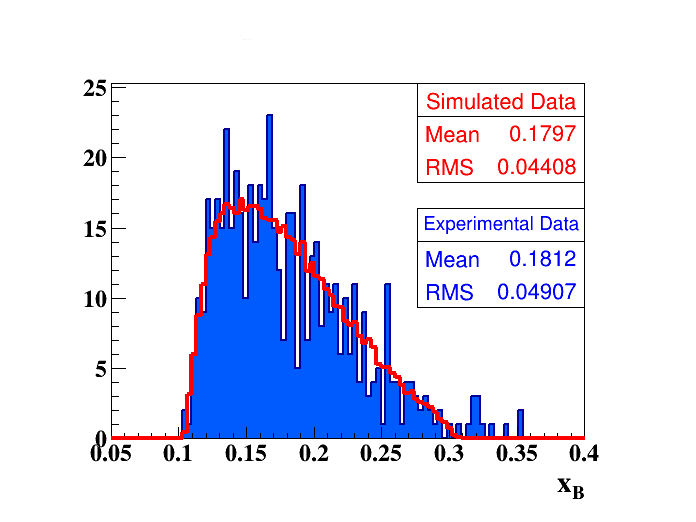
\includegraphics[trim=70 15 70 70,clip,width=6.3cm]{fig3/pi0/xB_Coh_pi0.png}
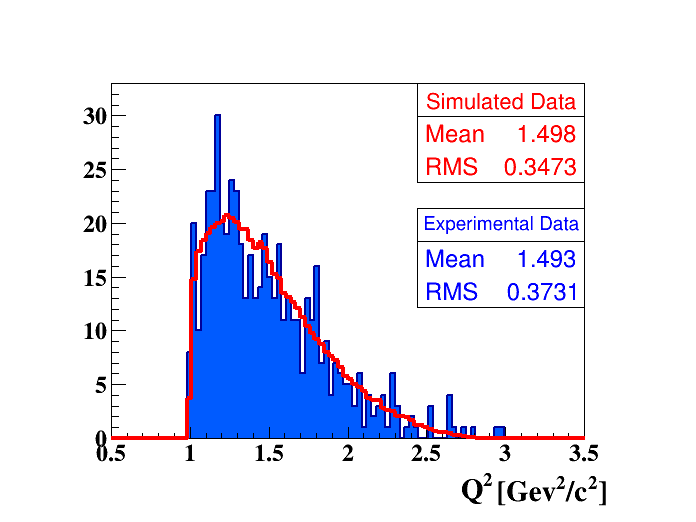
\includegraphics[trim=70 15 70 70,clip,width=6.3cm]{fig3/pi0/Q2_Coh_pi0.png}
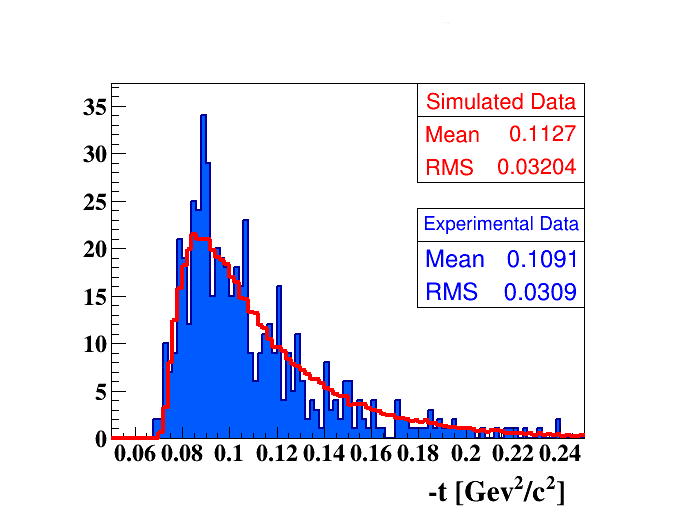
\includegraphics[trim=70 15 70 70,clip,width=6.3cm]{fig3/pi0/t_Coh_pi0.png}
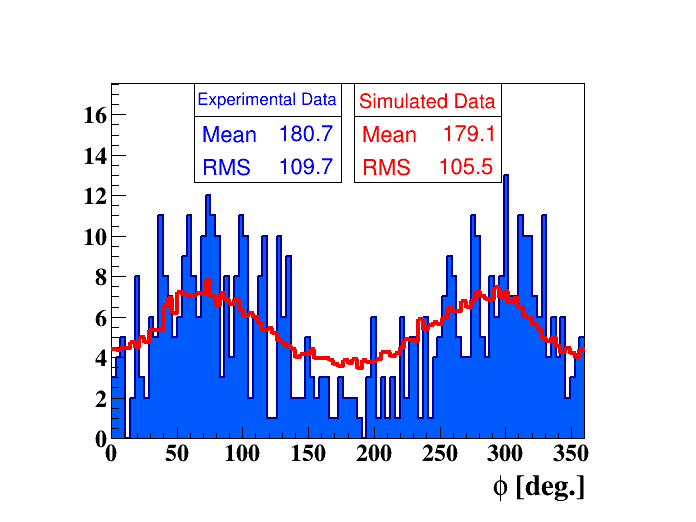
\includegraphics[trim=70 15 70 70,clip,width=6.3cm]{fig3/pi0/phi_h_Coh_pi0.png}
	\caption{The measured (filled blue) and simulated (red) distributions of
	coherent exclusive $\pi^0$ production as a function of $x$, $Q^2$, $-t$ and $\phi$.}
\label{fig:CohPi0Simul}
\end{figure}

\begin{figure}[p]
\center
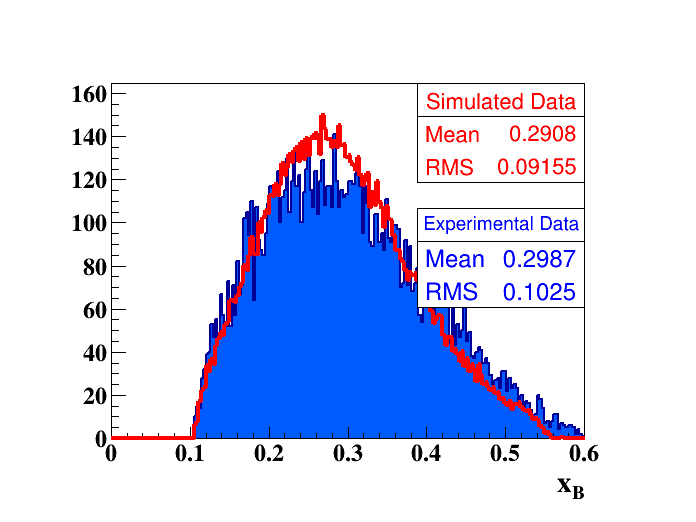
\includegraphics[trim=70 15 70 70,clip,width=6.3cm]{fig3/pi0/xB_InCoh_pi0.png}
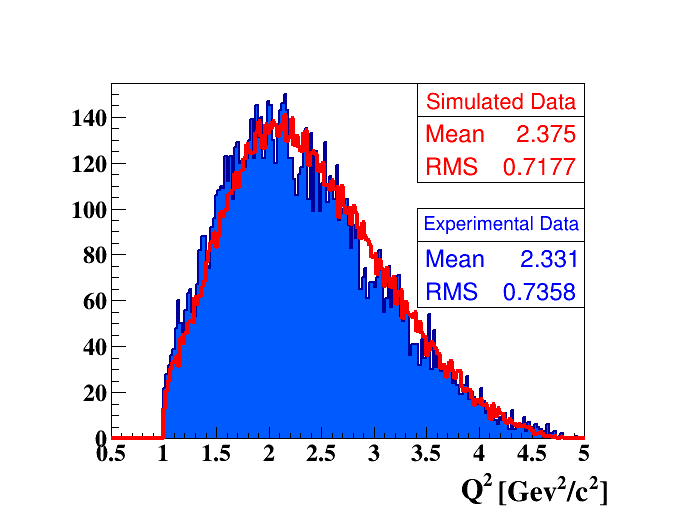
\includegraphics[trim=70 15 70 70,clip,width=6.3cm]{fig3/pi0/Q2_InCoh_pi0.png}
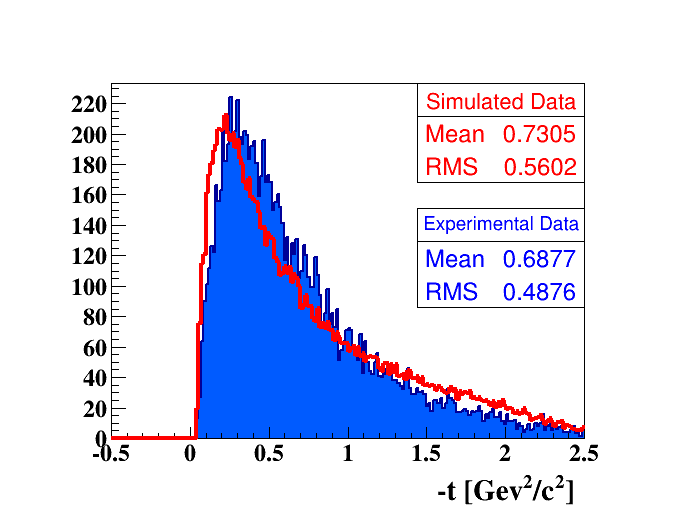
\includegraphics[trim=70 15 70 70,clip,width=6.3cm]{fig3/pi0/t_InCoh_pi0.png}
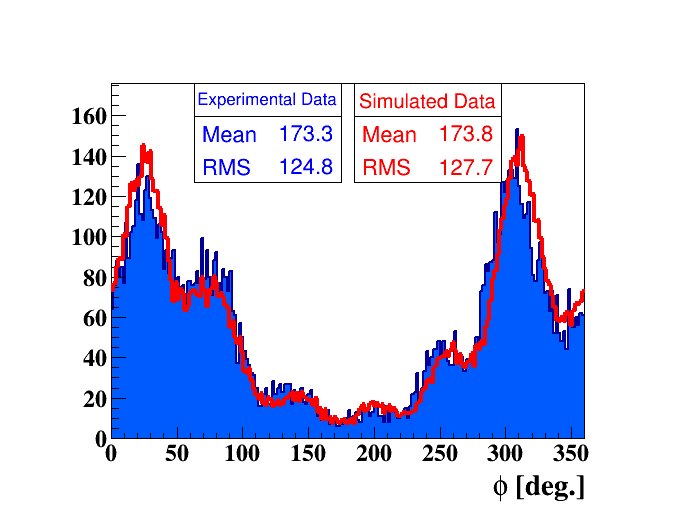
\includegraphics[trim=70 15 70 70,clip,width=6.3cm]{fig3/pi0/phi_h_InCoh_pi0.png}
	\caption{The measured (filled blue) and simulated (red) distributions of
	incoherent exclusive $\pi^0$ production as a function of $x$, $Q^2$, $-t$ and $\phi$.}
\label{fig:InCohPi0Simul}
\end{figure}


The $\pi^0$ contamination was found to be 2 to 4\% in the coherent channel and 3 to 17\% in the incoherent
channel (with variations between bins). To make the correction on the DVCS BSA, we assume that
the exclusive $\pi^0$ production has no such asymmetry. This has been checked with the exclusive 
$\pi^0$ production data, for which no significant level of BSA has been measured.

The second important source of background comes from accidentals. Despite the many exclusivity cuts, it is 
possible to have particles from different events getting combining and pass all the cuts and get 
into the data sample. To evaluate the number of such events, we invert the vertex selection 
of the two charged 
particles of the process, electron and helium (or proton in the incoherent case), and request that they
are separate. We find 4.1\% of the coherent and 6.5\% of the incoherent samples are accidentals. 

\subsection{Systematic errors}

To evaluate the systematic error of the measurement, we performed several specific studies. We 
evaluated the impact of changing the exclusivity selection cuts by varying them from 1 to 5 $\sigma$. 
We evaluated the impact of changing the binning in $\phi$ on the extraction of the beam-spin asymmetry
at 90°. We used the spread of the beam polarization measurements during the run period to evaluate their 
precision. We checked different methods to make the simulation of the exclusive $\pi^0$
production to evaluate the 
possible bias introduced by this correction. As radiative corrections are expected to be small
for our process, we did not apply them, but associated an error of their expected size.
These errors are summarized in Tab. \ref{Table:systematic_uncertainties}, with their respective 
evaluated sizes. They are added quadratically for the total systematic error presented in the results.

\begin{table}[tbp]
\begin{center}
	\begin{tabular}{|m{4cm}|m{2cm}<{\centering}|m{2.3cm}<{\centering}|m{3.7cm}<{\centering}|}
\hline
\bf Systematic source & \bf  Coherent channel  & \bf Incoherent channel & \bf Type of systematic 
error\\
\hline
DVCS cuts & 8 $\%$ &  6 $\%$ & bin to bin\\
\hline
Data binning & 5.1$\%$ & 7.1$\%$ &bin to bin\\
\hline
Beam polarization &  3.5$\%$ &  3.5$\%$& Normalization\\
\hline
$\pi^0$ subtraction &  0.6$\%$ &  2.0$\%$ &bin to bin\\
\hline
%Beam charge asymmetry &  ~~~~~1.1$\%$&  ~~~~~1.1$\%$\\
%\hline
Radiative corrections &  0.1$\%$ & 0.1$\%$ & bin to bin\\
\hline
\textbf{Total} &  \textbf{10.1}$\%$ &   \textbf{10.1}$\%$ &bin to 
bin\\
\hline
\end{tabular}
\caption{The systematic uncertainties on the measured coherent and incoherent 
beam-spin asymmetries at $\phi = 90^{\circ}$.}
\label{Table:systematic_uncertainties}
\end{center}
\end{table}

%TODO MAke sure acceptance ratio is indeed pi0

As discussed above, the best way to define $t$ in the incoherent channel is not completely
straightforward. As can be seen in the Fig. \ref{fig:InCohDiag}, 
we can either use $t$ or $t^\prime$ ($= (p - p^\prime)^2$). In principle, the two are 
identical, but experimentally we face some issues. The measurement of $t$ is less precise than
$t^\prime$ because it involves the photon rather than charged particles. However, the 
exact measurement of $t^\prime$ is impossible and one needs to assume a proton at rest
in the initial state to calculate $t^\prime$. As it is not obvious which solution is best,
we studied the difference between them by analyzing the data independently using the two 
definitions. We found no significant difference between them, as is 
illustrated in Fig. \ref{fig:ttpComp}. We use in our final results $t$,
which is the correct definition.

\begin{figure}[tbp!]
\center
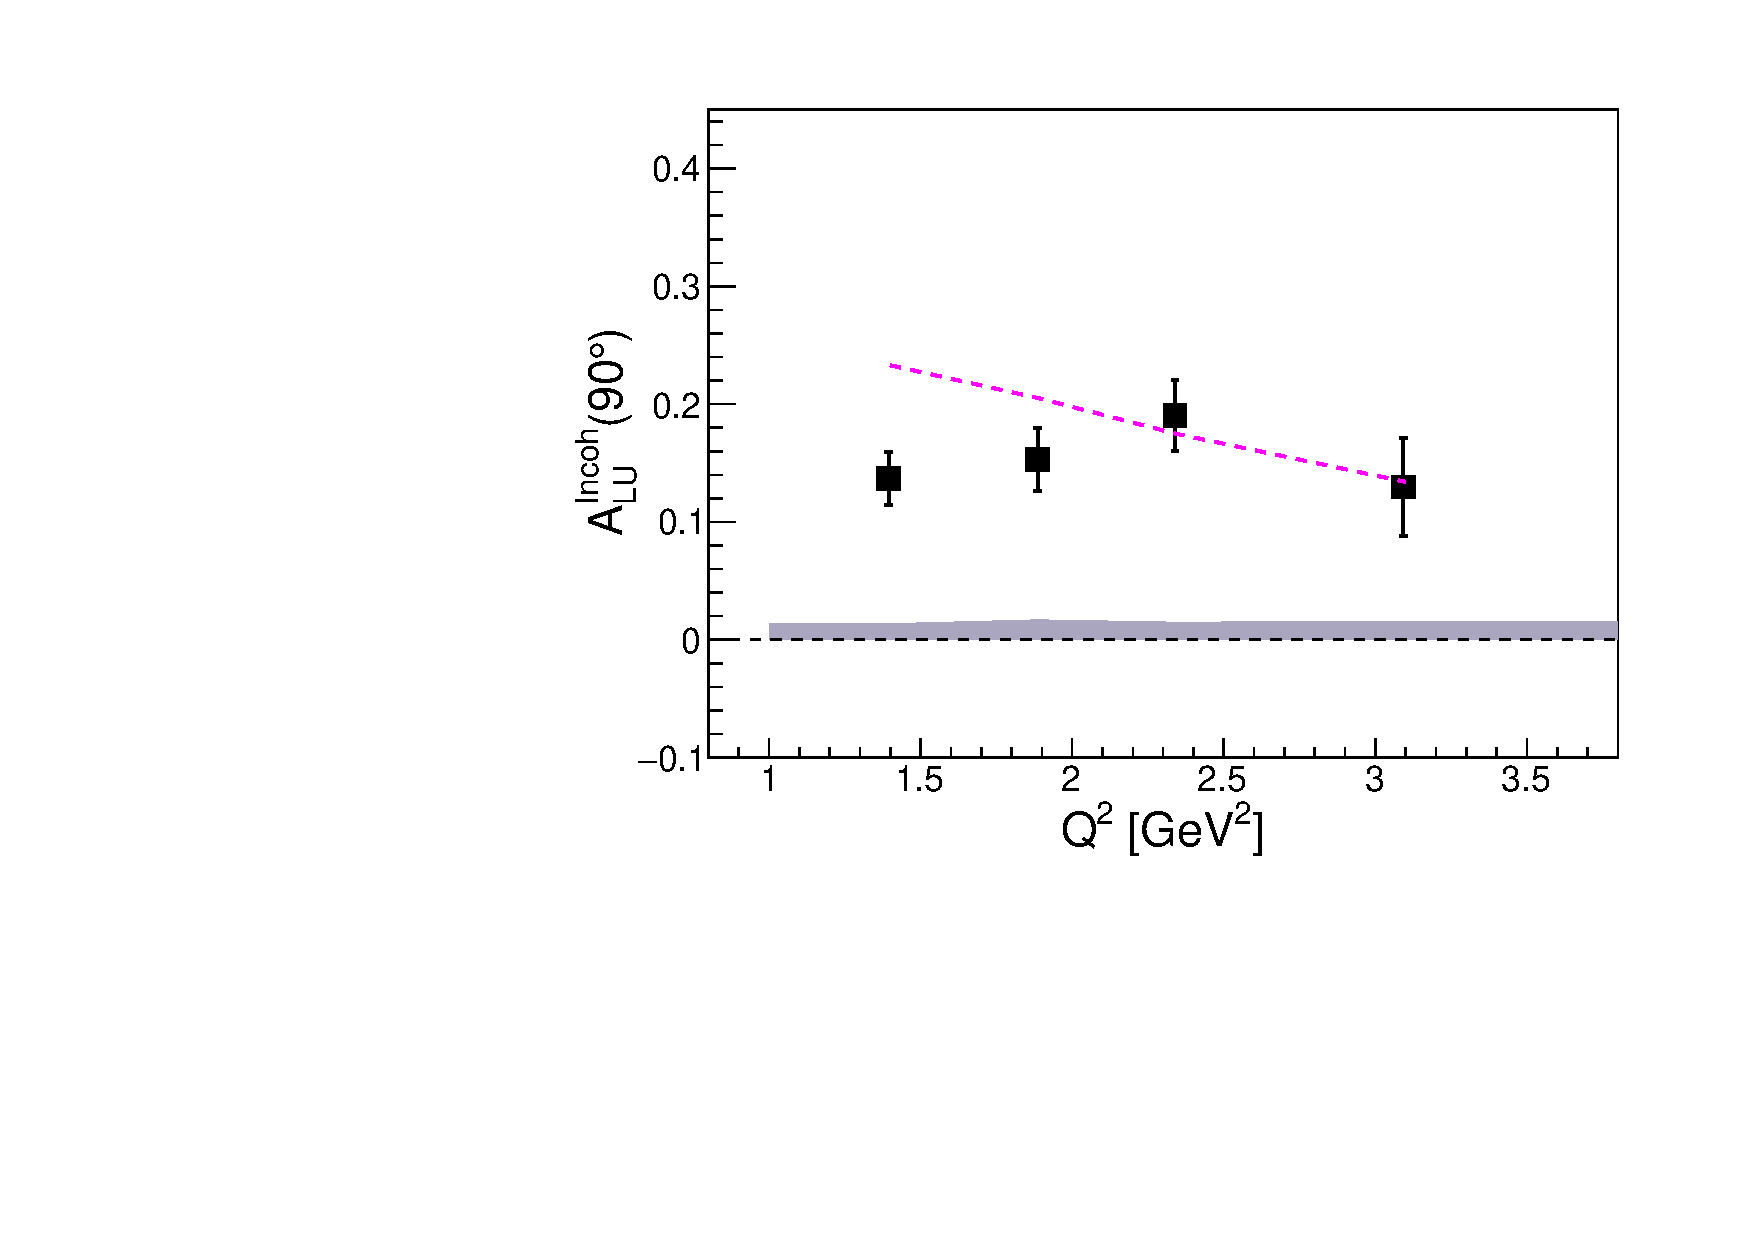
\includegraphics[width=7.4cm]{fig3/ALU_90_p_vs_Q2_shortscenrario.pdf}
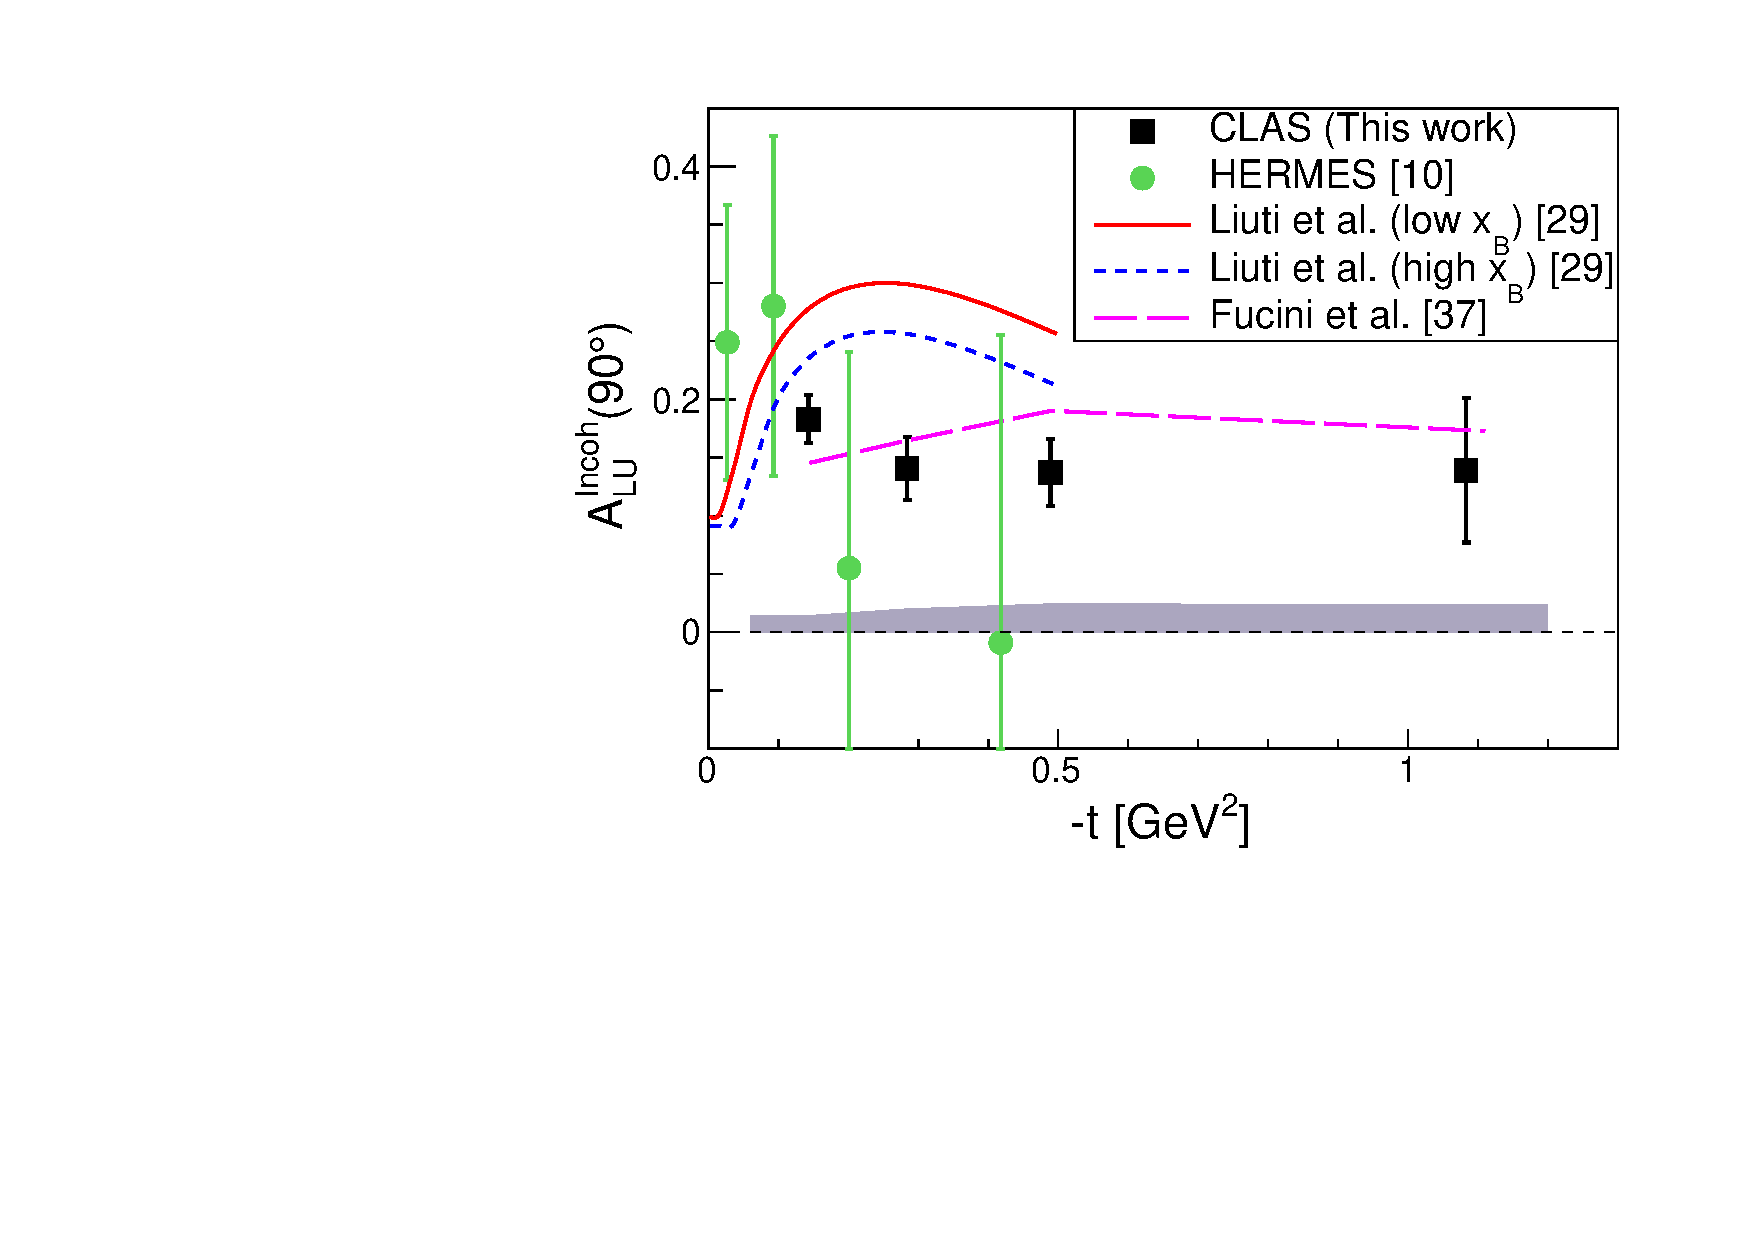
\includegraphics[width=7.4cm]{fig3/ALU_90_p_vs_t_shortscenrario.pdf}
%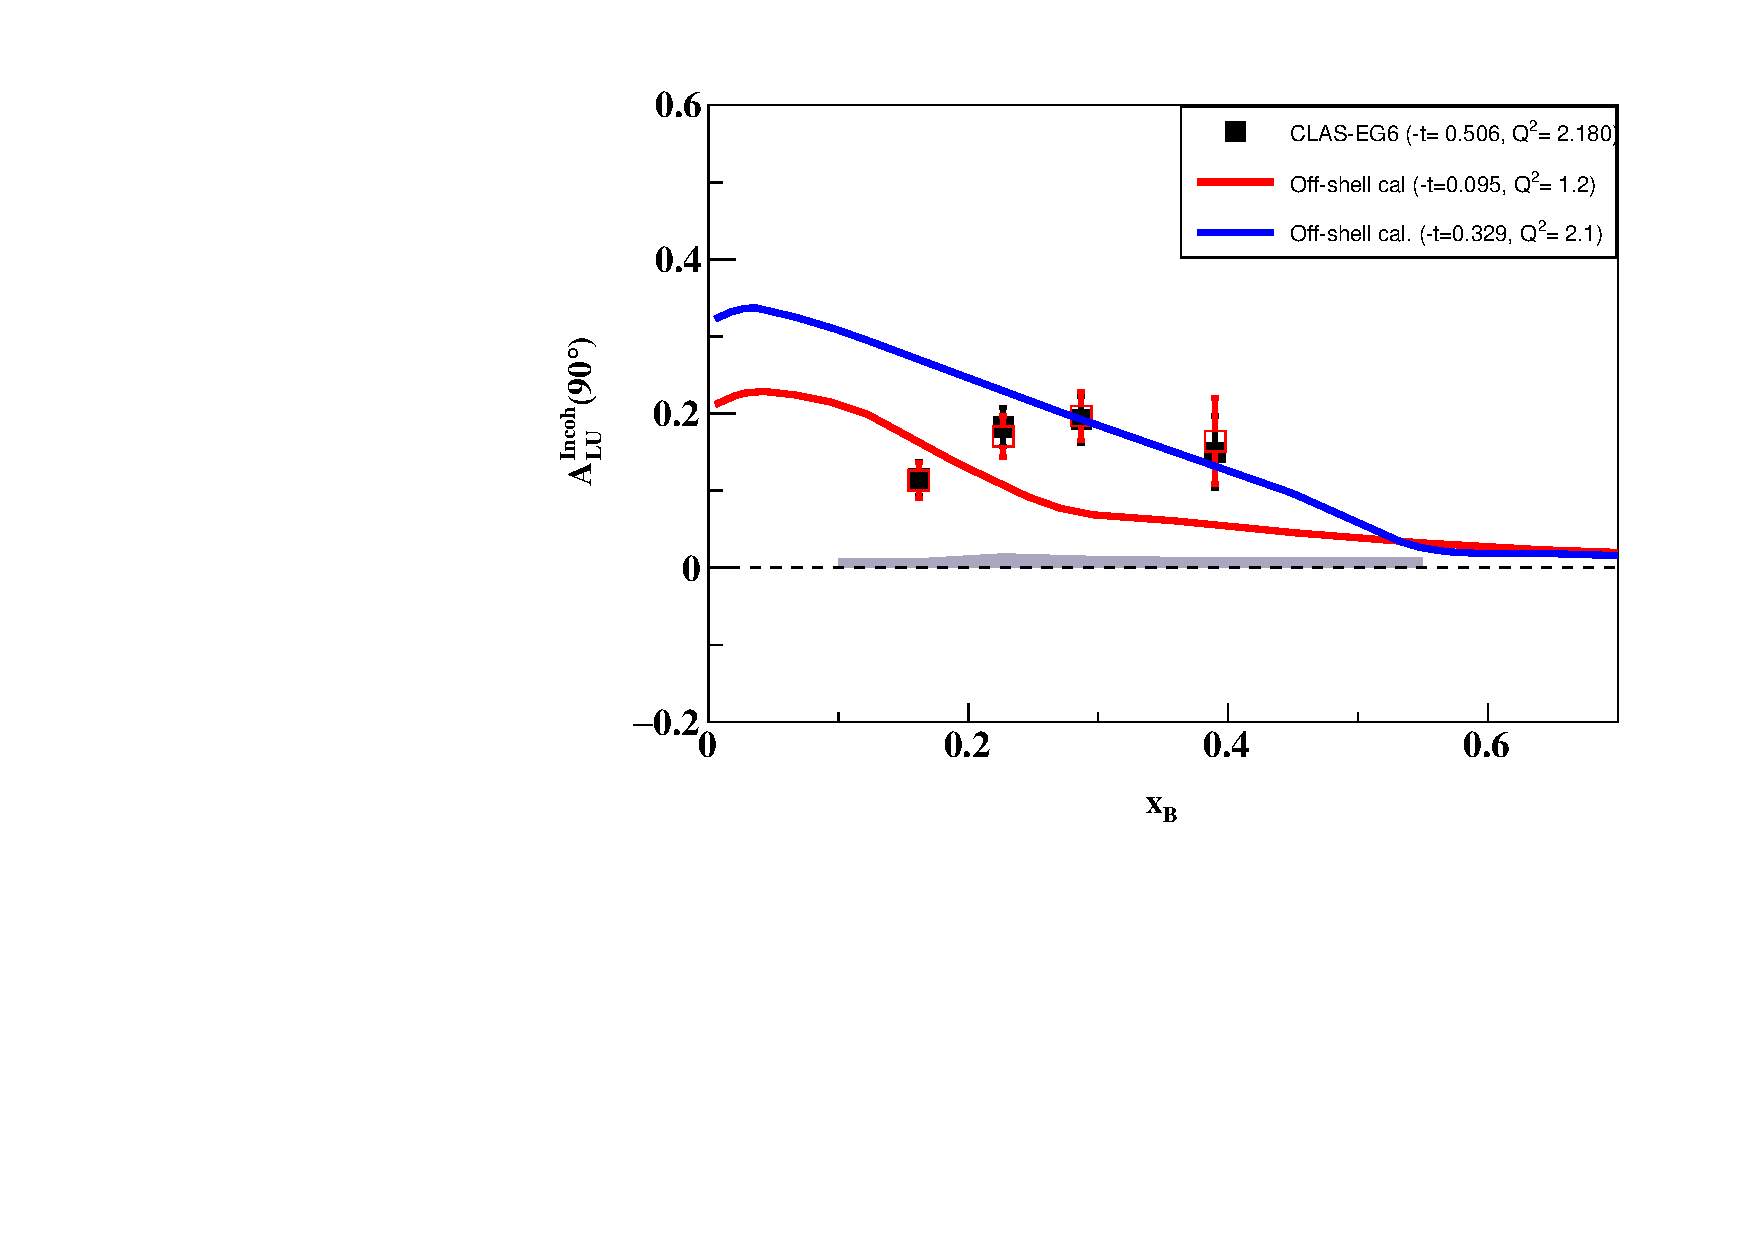
\includegraphics[width=7cm]{fig3/ALU_90_p_vs_x_shortscenrario.pdf}
	\caption{The BSA at 90° ($A_{LU}^{Incoh} (90^\circ)$) as a
	function of $Q^2$ and $-t$, using the photon based $t$ definition (empty red)
	and the proton based $t^\prime$ definition (full black).}
	%TODO we could remove HERMES and the models on these
\label{fig:ttpComp}
\end{figure}

\section{Results}

\subsection{Coherent DVCS}

In Fig. \ref{fig:CohALUphi}, we present the results for the BSA in the coherent DVCS channel. We 
observe the dominant sinusoidal component typical of the DVCS BSA, but note also the large size 
of the asymmetry, almost double than the one measured for the free proton \cite{Jo:2015ema}. This 
predicted feature of nuclear DVCS \cite{Guzey:2003jh} is observed here for the first time, we
can conclude that this measurement cleanly isolates the coherent DVCS process. The absence of 
this feature in HERMES data and its clear observation here indicates that the recoil 
detection is a strong help to isolate the effects of the coherent DVCS process from backgrounds. 

\begin{figure}[bp!]
\center
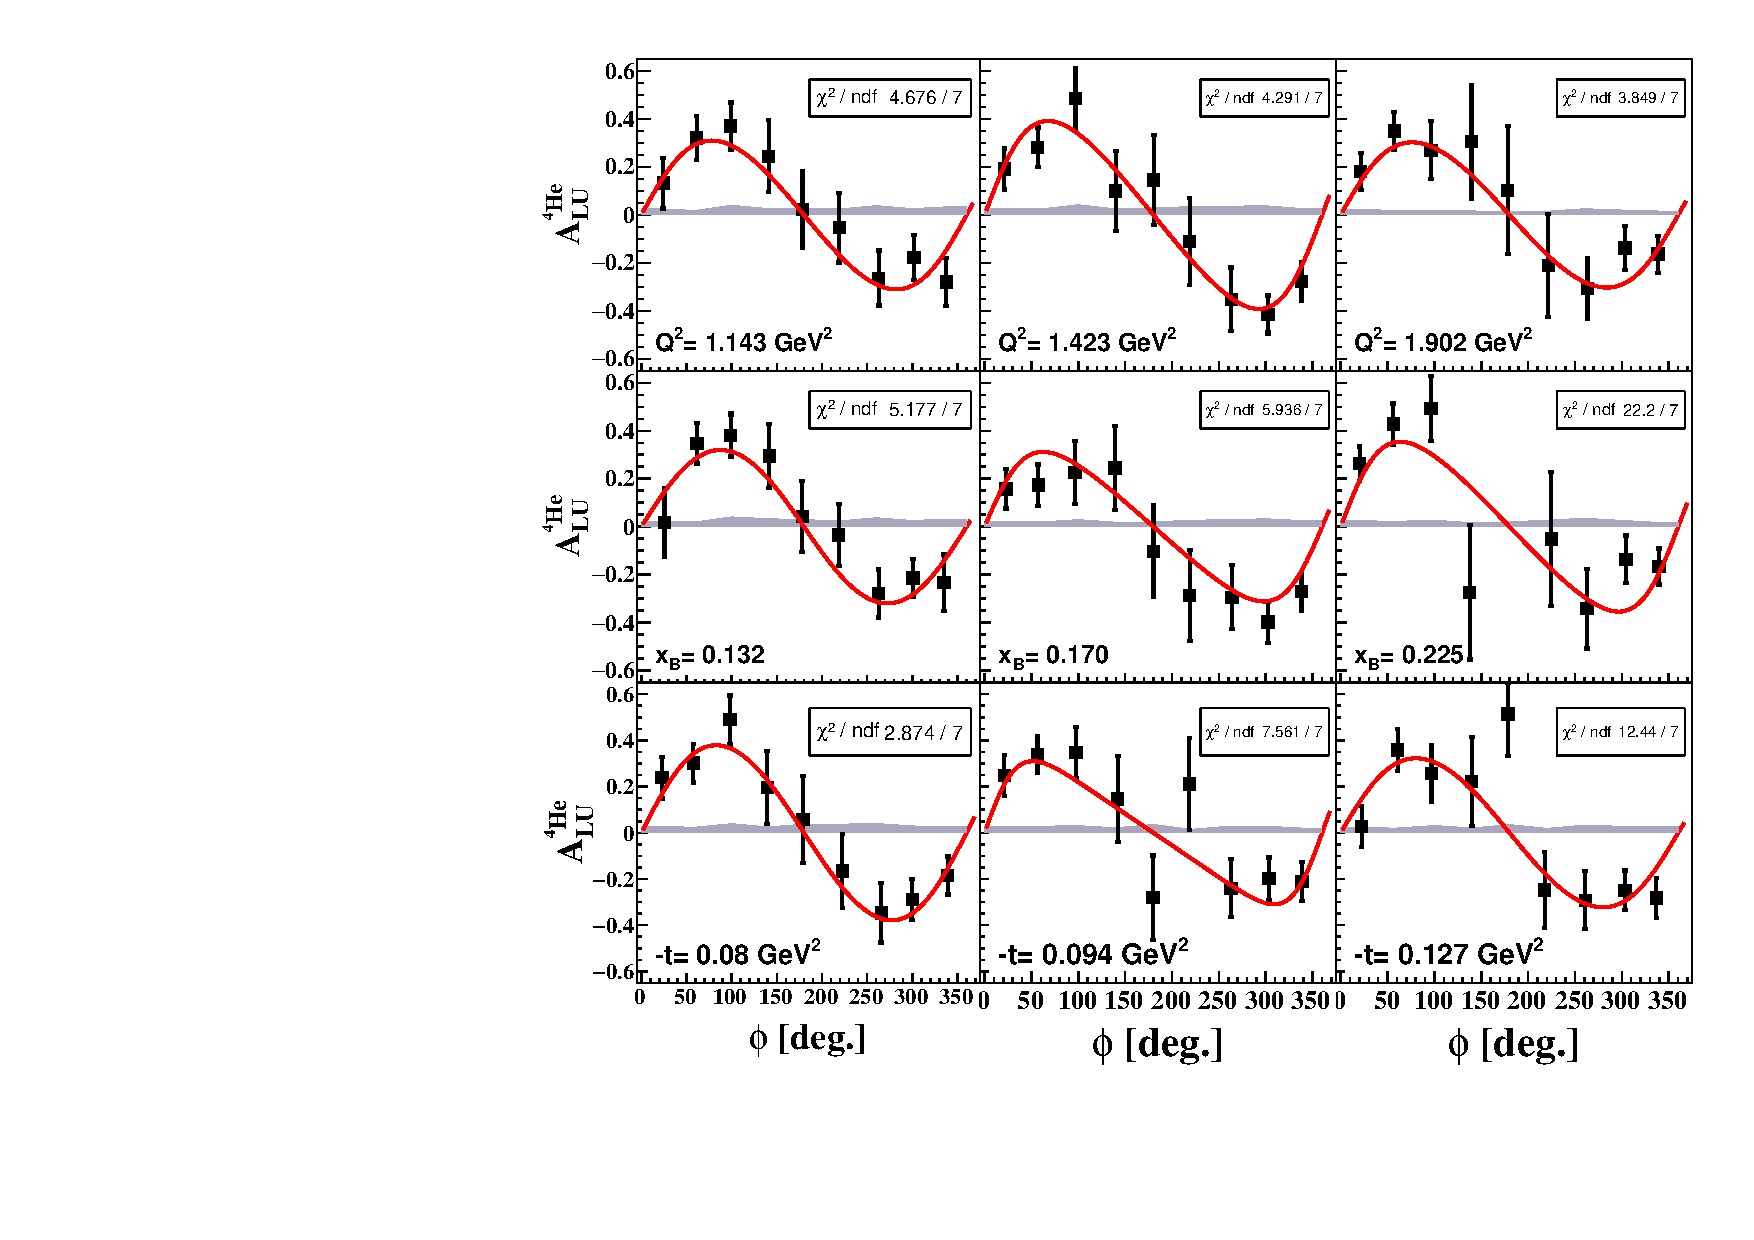
\includegraphics[width=12cm]{fig3/Coherent_ALU_phi.pdf}
	\caption{The BSA in the coherent exclusive photo-production off helium-4 as a 
	function of $\phi$ and $Q^2$ 
	(top panels), $x$ (middle panels) and $-t$ (lower panels). Error bars are  
	statistical, Grey bands represent the systematic errors. The data is fitted with Eq. 
	\ref{eq:A_LU-coh}, the results of these fits are drawn with red full lines.}
\label{fig:CohALUphi}
\end{figure}

\begin{figure}[tbp]
\center
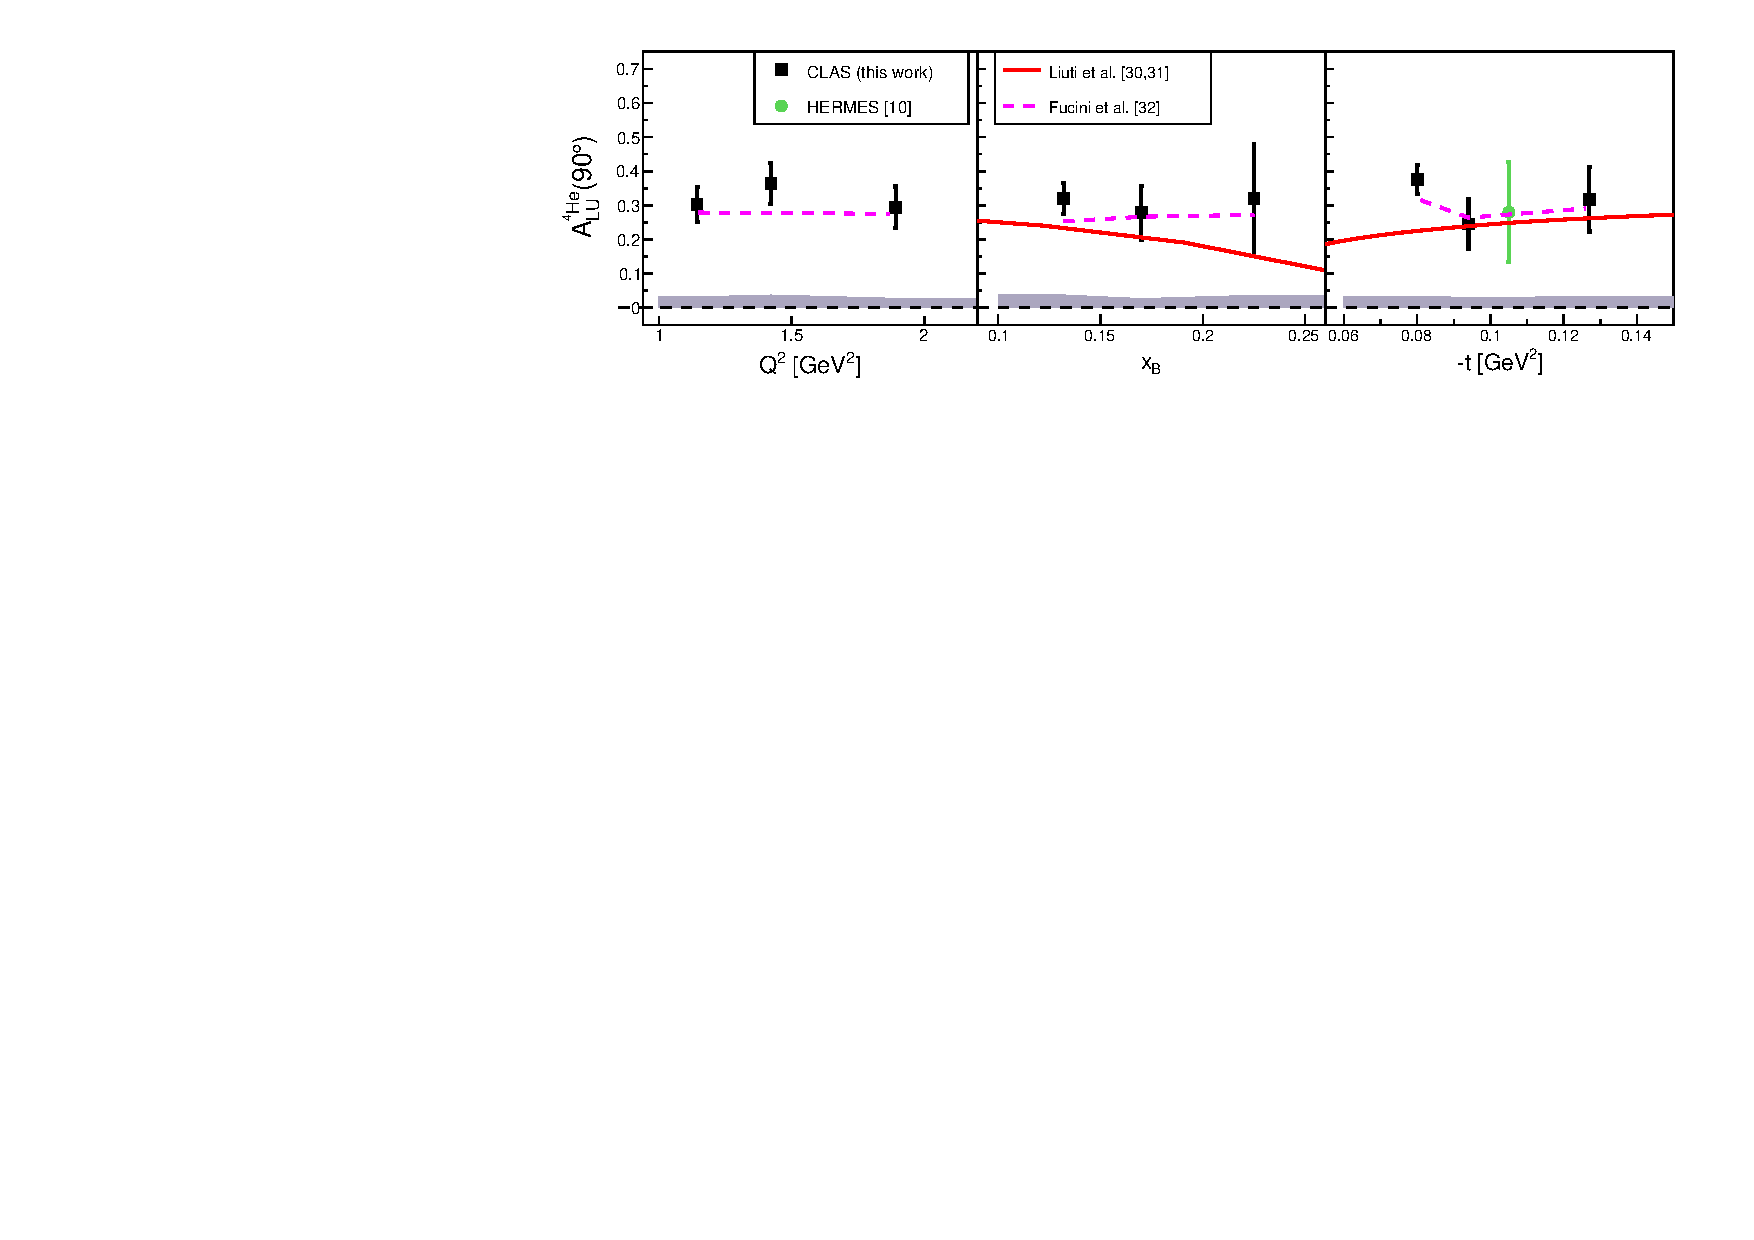
\includegraphics[width=10cm]{fig3/Coherent_ALU_phi_90.pdf}
\caption{The BSA at 90° as a function of $Q^2$ (top panel), $x$ (middle panel) and $-t$ (lower panel).
	Our results are shown with black squares, HERMES results 
	with green circles \cite{Airapetian:2009cga} and theoretical predictions 
	from \cite{Liuti:2005gi} with full and dashed lines.}
\label{fig:CohALU90}
\end{figure}

In order to compare to models, we extract the BSA at 90° in Fig. \ref{fig:CohALU90}. The model 
compared to the data \cite{Liuti:2005gi} is based on the idea that the main nuclear effects are 
included by accounting for the nucleon off-shellness and kinematics in nuclei with a nuclear
spectral function. It appears that the model undershoot our results systematically. However, 
a more recent calculation, using similar principles but with a more advanced nuclear spectral 
function \cite{Fucini:2018gso} has been able to reproduce the data very well. This 
sort of theoretical model, also able to describe the EMC effect, is the only one which has 
been confronted to this data yet. We observe that reproducing these data is not 
straightforward and necessitates an advanced nuclear model.

% TODO add footnote
%\footnote{We actually show here the opposite of HERMES results, as the HERMES 
%experiment ran with a positron beam, which lead to opposite BSAs.}
%TODO Add Sergio's results there

One of the promise of the helium-4 DVCS was the expected ease to extract the CFF $\mathcal{H}_A$ from
data. To do so, we used the form from Eq. \ref{eq:A_LU-coh} to fit the data from Fig. 
\ref{fig:CohALUphi}. We obtained the real and imaginary parts of the unique helium-4
CFF presented in Fig. \ref{fig:CohCFF}. The results are rather encouraging, the two parts
of the CFF are constrained by data without need of any model. This capacity to obtain a
model independent result with such a limited data set offers a striking contrast with the
situation of the free proton fits described in Chap. \ref{chap:pheno}.

\begin{figure}[tbp!]
\center
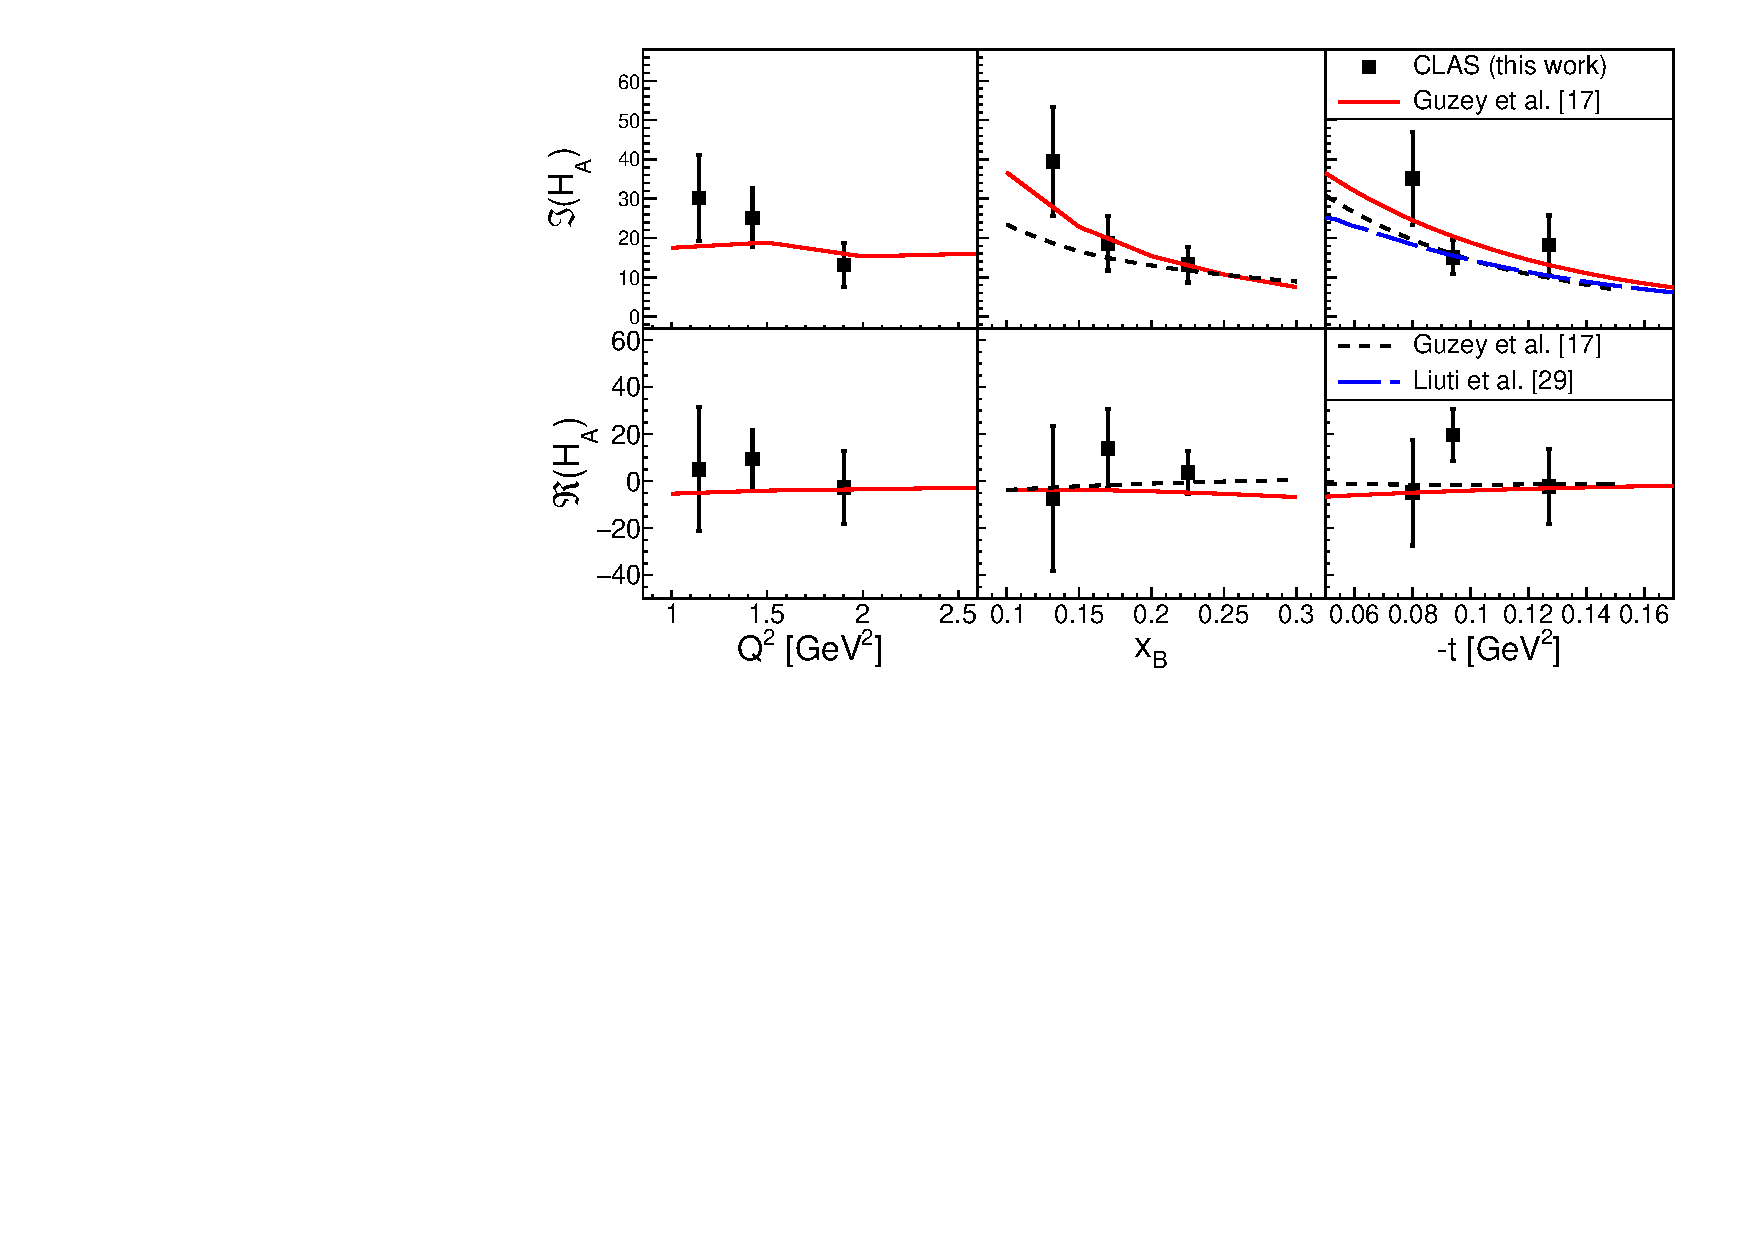
\includegraphics[width=14cm]{fig3/Coherent_CFF.pdf}
	\caption{The imaginary (top panels) and real (bottom panels) parts of the helium-4
	CFF $\mathcal{H}_A$ as a function of $Q^2$ (left panels), $x$ (middle panels) and 
	$-t$ (right panels). The red full line red is the theoretical calculation from 
	\cite{Guzey:2003jh,Guzey:2008th}, the black dashed line is the same calculation 
	using the VGG model as input \cite{Vanderhaeghen:1999xj,Guidal:2004nd}, and
	the blue dashed line is a calculation from \cite{GonzalezHernandez:2012jv}.} 
	%TODO change model names description
\label{fig:CohCFF}
\end{figure}

The CFF extraction allows us to compare the results to other theoretical calculations.
The calculation within the impulse approximation from \cite{Guzey:2003jh,Guzey:2008th} 
gives the nuclear GPD directly
from the proton and neutron GPDs, such that it allows to test the effect of different 
nucleon's GPD models. In Fig. \ref{fig:CohCFF}, we can see that the effect of such a change of 
GPD model is of similar size or larger than the difference with another nuclear 
model \cite{GonzalezHernandez:2012jv}. However, at the level of precision of the present data,
it is not possible to resolve which variant is best. This feature still highlights the 
importance to try different nucleon models when evaluating a feature of the data.

This measurement of the BSA in the deeply virtual coherent exclusive photo-production on a nucleus
is the first to clearly isolate the effect of coherent nuclear DVCS and of nuclear GPDs. While, the
statistical precision and the kinematic coverage are still far behind the experimental results on
proton target, the results appear to match very well the predictions using the GPD framework. It 
validates the relevance of the nuclear DVCS to study the nucleus globally in terms of quarks and 
gluons, bypassing any intermediate degree of freedom like the nucleons. 

\subsection{Incoherent DVCS}

\begin{figure}[bp!]
\center
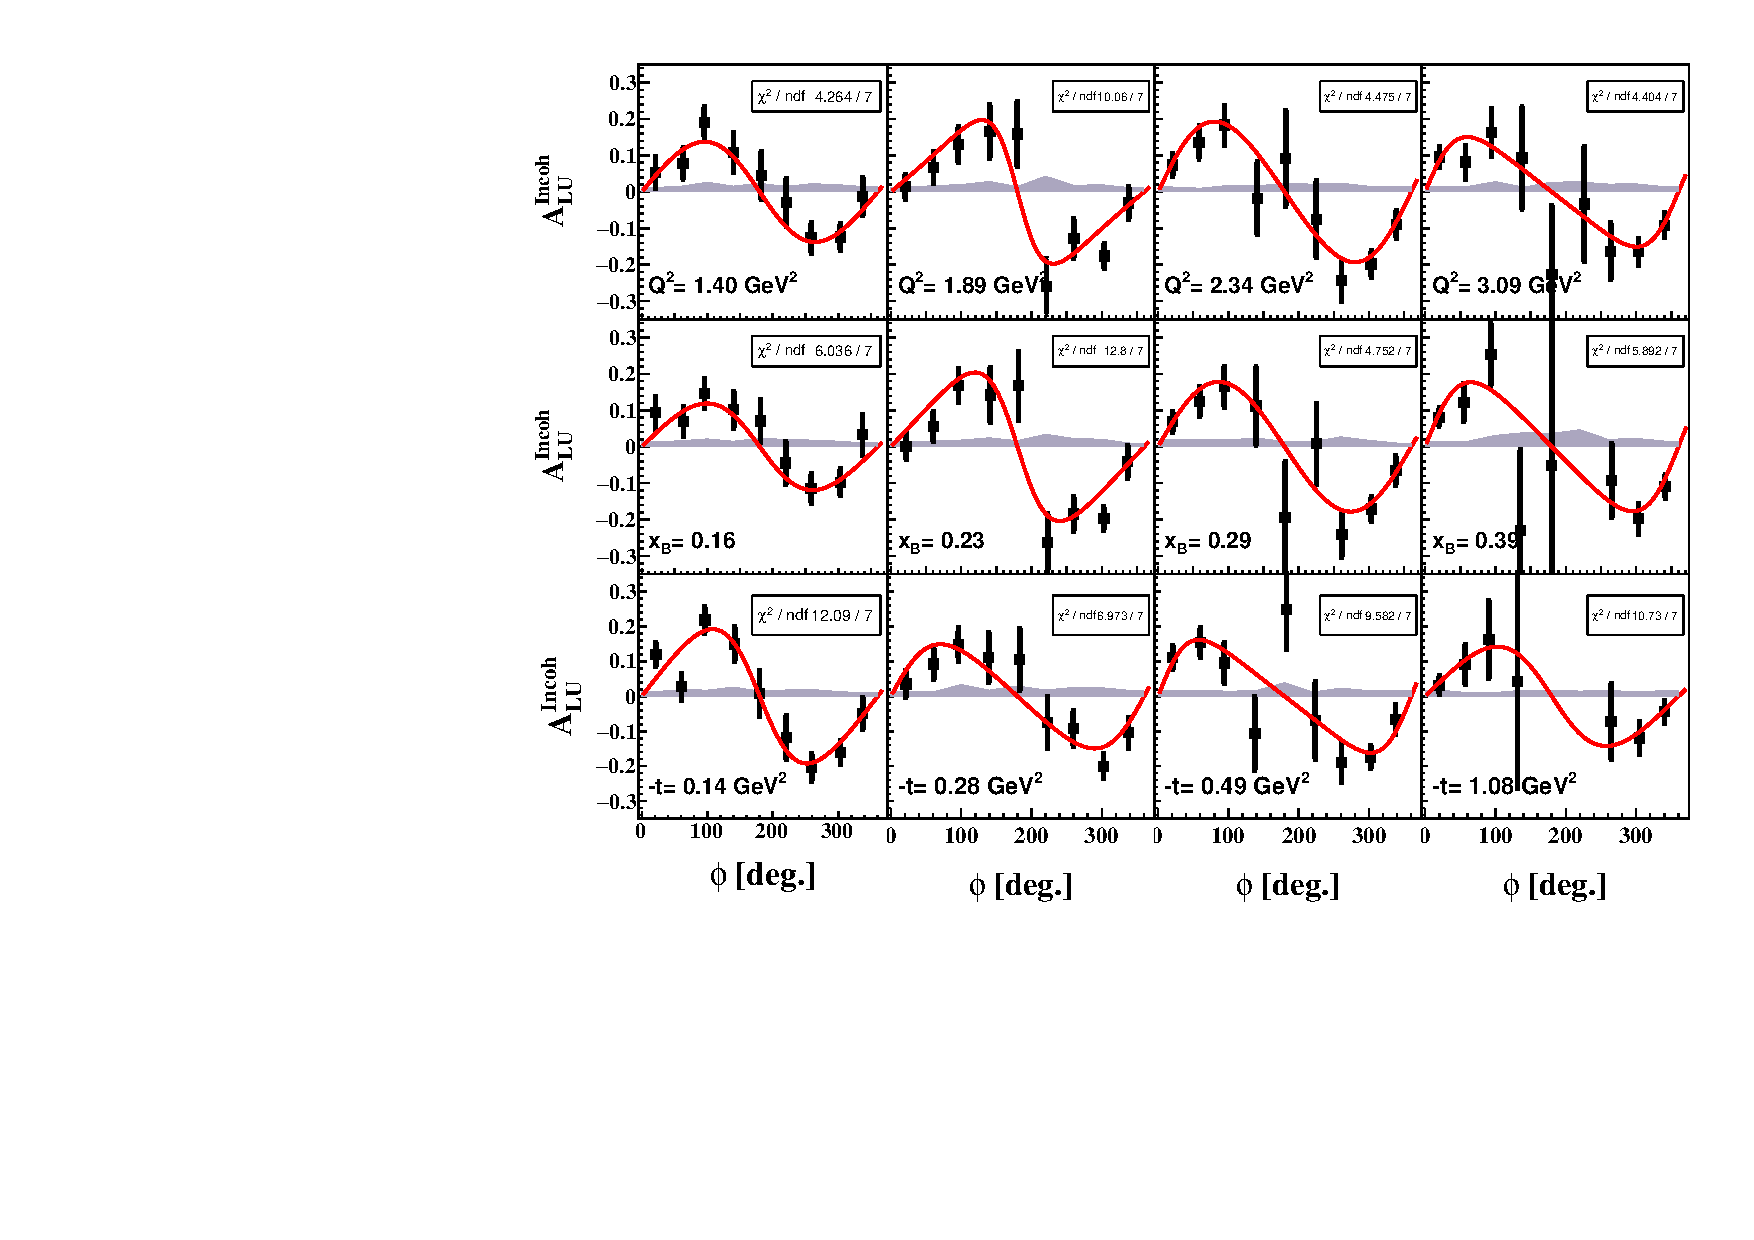
\includegraphics[width=15cm]{fig3/incoherent_ALU_phi.pdf}
	\caption{The BSA in the incoherent exclusive photo-production off a proton bound in
	helium-4 as a function of $\phi$ and $Q^2$ 
	(top panels), $x$ (middle panels) and $-t$ (lower panels). Error bars are  
	statistical, Grey bands represent the systematic errors. The data is fitted with the 
	form $\frac{\alpha \sin(\phi)}{1+\beta \cos(\phi)}$; the results of the 
	fits are drawn with black full lines.}
\label{fig:InCohALUphi}
\end{figure}

The results for the measurement of the BSA in the incoherent DVCS channel are presented in
Fig. \ref{fig:InCohALUphi}. They display patterns rather similar to the one observed with the 
free proton, with a clear domination of their sinusoidal component. To compare the data to 
models, we extract the BSA at 90° with a fit of the form $\frac{\alpha \sin(\phi)}{1+\beta \cos(\phi)}$. 

The asymmetries at 90° are presented in Fig. \ref{fig:IncALU} together with the theoretical
calculation presented also in Fig. \ref{fig:CohALU90}. The results are much more precise than 
the existing HERMES data and offer a strong constraint on the model presented. As in the
coherent case, the calculation appears to have issues to reproduce the shape of the data.
However, this time the calculation overshoots the data, sometimes by a significant amount.
An interesting way to look into this issue is to show the result on incoherent DVCS compared 
with the free proton. We can for instance make a ratio, in a fashion similar to the EMC 
effect, which allows to cancel out
the effects from the nucleon structure and highlight nuclear effects. Such ratio is presented
in Fig. \ref{fig:IncRatios}, where we observe again that most models overshoot the data.


\begin{figure}[tbp!]
\center
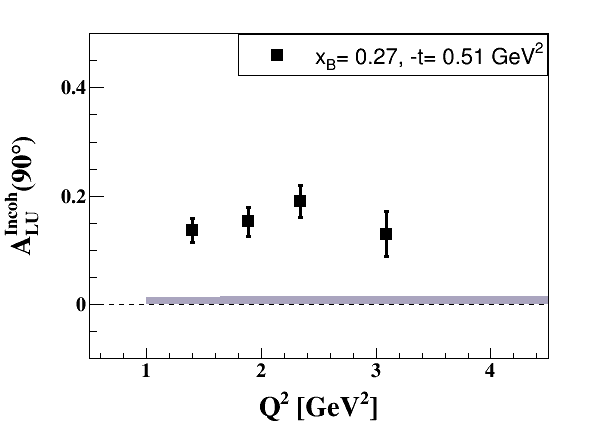
\includegraphics[width=7.4cm]{fig3/ALU_90_p_vs_Q2_shortscenrario.png}
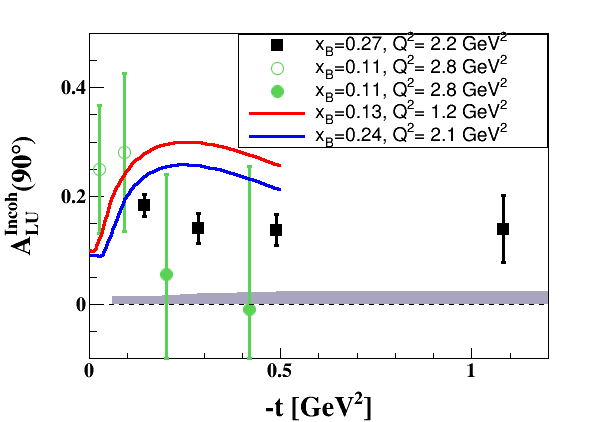
\includegraphics[width=7.4cm]{fig3/ALU_90_p_vs_t_shortscenrario.png}
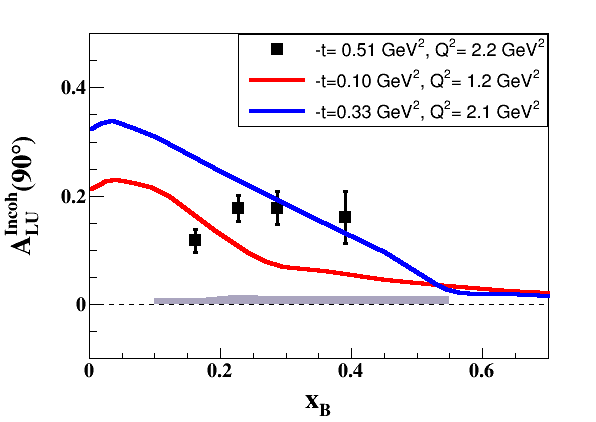
\includegraphics[width=7.4cm]{fig3/ALU_90_p_vs_x_shortscenrario.png}
	\caption{The BSA at 90° as a function of  $Q^2$ (top left), $x$ (top right) and 
	$-t$ (bottom). Our measurement is represented with black squares, HERMES 
	measurement \cite{Airapetian:2009cga} with green circles and the theoretical 
	calculation from \cite{Liuti:2005gi} with full lines.}
\label{fig:IncALU}
\end{figure}

\begin{figure}[tbp!]
\center
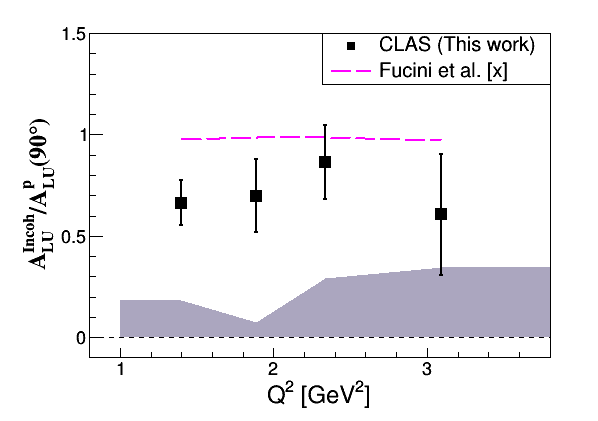
\includegraphics[width=7.4cm]{fig3/ALU_ratioInc_Q2_shortscenrario.png}
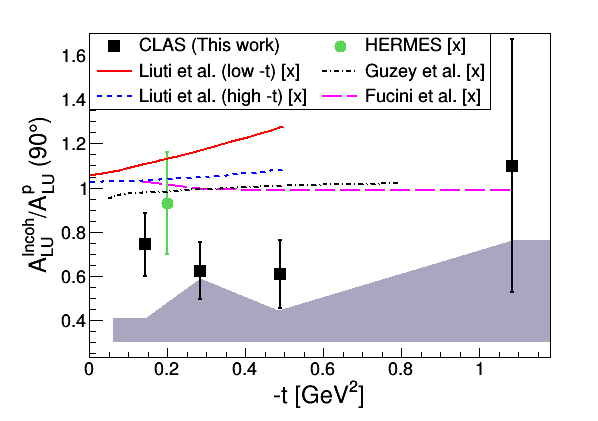
\includegraphics[width=7.4cm]{fig3/ALU_ratioInc_t_shortscenrario.png}
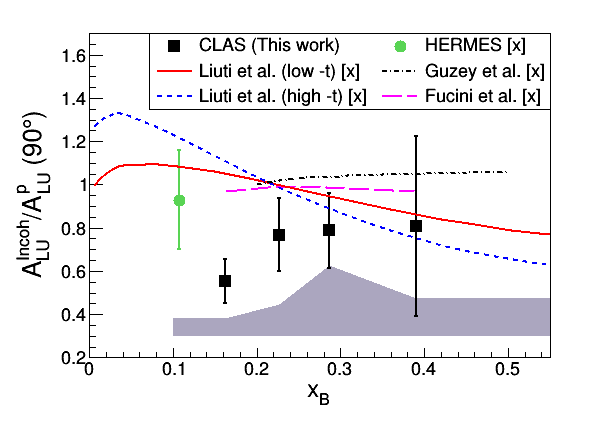
\includegraphics[width=7.4cm]{fig3/ALU_ratioInc_x_shortscenrario.png}
	\caption{DVCS BSA ratio of the bound proton to the free proton as a function of 
	$Q^2$ (top left), $x$ (top right) and $-t$ (bottom). The present measurement is 
	represented with black squares, HERMES 
	measurement \cite{Airapetian:2009cga} with green circles, the theoretical 
	calculation from \cite{Liuti:2005gi} with blue and red full lines and the
	calculation from \cite{Guzey:2008fe} with full and dashed black lines.}
\label{fig:IncRatios}
\end{figure}

This measurement of the incoherent DVCS BSA shows a global tendency of the experimental data 
to be smaller than expected from theoretical calculations. We observe the incoherent DVCS 
BSA to go as low as 60\% of the size of the BSA observed
on the free proton. This drastic reduction is still unexplained, though some theoretical 
work has been recently published to prolong the calculation from \cite{Fucini:2018gso} to the incoherent 
channel \cite{Fucini:2019xlc}. The explanation for this surprising behavior can come from different sources
both in the initial state and the final state.

\section{Summary}


% \begin{figure}
% \includegraphics{}%
% \caption{\label{}}
% \end{figure}

% Surround figure environment with turnpage environment for landscape
% figure
% \begin{turnpage}
% \begin{figure}
% \includegraphics{}%
% \caption{\label{}}
% \end{figure}
% \end{turnpage}

% tables should appear as floats within the text
%
% Here is an example of the general form of a table:
% Fill in the caption in the braces of the \caption{} command. Put the label
% that you will use with \ref{} command in the braces of the \label{} command.
% Insert the column specifiers (l, r, c, d, etc.) in the empty braces of the
% \begin{tabular}{} command.
% The ruledtabular enviroment adds doubled rules to table and sets a
% reasonable default table settings.
% Use the table* environment to get a full-width table in two-column
% Add \usepackage{longtable} and the longtable (or longtable*}
% environment for nicely formatted long tables. Or use the the [H]
% placement option to break a long table (with less control than 
% in longtable).
% \begin{table}%[H] add [H] placement to break table across pages
% \caption{\label{}}
% \begin{ruledtabular}
% \begin{tabular}{}
% Lines of table here ending with \\
% \end{tabular}
% \end{ruledtabular}
% \end{table}


% Specify following sections are appendices. Use \appendix* if there
% only one appendix.
%\appendix
%\section{}

% Surround table environment with turnpage environment for landscape
% table
% \begin{turnpage}
% \begin{table}
% \caption{\label{}}
% \begin{ruledtabular}
% \begin{tabular}{}
% \end{tabular}
% \end{ruledtabular}
% \end{table}
% \end{turnpage}

\begin{acknowledgments}
 Put your acknowledgments here.
\end{acknowledgments}

% Create the reference section using BibTeX:
\bibliography{basename of .bib file}

\end{document}

